\documentclass{ltjsarticle}

%%%%%%%%%%packages%%%%%%%%%%
%% colors and links
\usepackage[svgnames]{xcolor}
\usepackage[colorlinks,citecolor=DarkGreen,linkcolor=Blue,linktocpage,unicode]{hyperref} 

%% equations
%%%% math
\usepackage{amsmath,amsfonts,amssymb,amsthm}
\usepackage{mathtools}
\usepackage{mathrsfs}
\usepackage{bm}
\usepackage{cancel}
\usepackage{dsfont}
%%%% physics
\usepackage{siunitx}
\usepackage{physics}
%% positioning
\usepackage{array}
\usepackage{float}

%% table
\usepackage{booktabs}
\usepackage{multirow}
\usepackage{hhline}
\usepackage{caption}
\captionsetup{format=hang}
\usepackage{subcaption}

%% figure
\usepackage{graphicx}
\usepackage{tikz}
\usepackage{circuitikz}

%% decorations
\usepackage{titlesec}
\usepackage{picture}

%% framing
\usepackage{fancybox}
\usepackage{boites}
\usepackage{tcolorbox}
\tcbuselibrary{skins,theorems,breakable}

%% citation
\usepackage{cite}

%%%%%%%%%%optional settings%%%%%%%%%%

%%%%%図表並列%%%%%
\makeatletter
\newcommand{\figcaption}[1]{\def\@captype{figure}\caption{#1}}
\newcommand{\tblcaption}[1]{\def\@captype{table}\caption{#1}}
\makeatother

%%%%%itemization%%%%%
\renewcommand{\labelenumi}{\theenumi}
\renewcommand{\theenumi}{(\arabic{enumi})} % 箇条書きをローマ数字に

%%%%%%theorem environments%%%%%
\newtheoremstyle{mystyle}%   % スタイル名
    {}%                      % 上部スペース
    {}%                      % 下部スペース
    {\normalfont}%          % 本文フォント
    {}%                      % インデント量
    {\bf}%                  % 見出しフォント
    {.}%                      % 見出し後の句読点
    {\newline}%                     % 見出し後のスペース
    {\underline{\thmname{#1}\thmnumber{#2}\thmnote{(#3)}}}%
    % 見出しの書式 (can be left empty, meaning `normal')
\theoremstyle{mystyle} % スタイルの適用

\newtheorem{theorem}{定理}[section]
\newtheorem{definition}{定義}[section]
\newtheorem{proposition}[definition]{命題}
\newtheorem{corollary}[theorem]{系}
\renewcommand{\proofname}{証明}

\newtheorem{remark}{Remark. }[section]
\newtheorem{axiom}{公理}[section]
\newtheorem{conjecture}{Conjecture. }[section]

%%%%%%mathtools%%%%%
\mathtoolsset{showonlyrefs=true} % 被参照数式のみ数式番号割り振り
\numberwithin{equation}{section}

\makeatletter
\@addtoreset{equation}{section}
\makeatother

%%%%%%framing%%%%%

\newcommand{\lto}{\longrightarrow}
\newcommand{\lmto}{\longmapsto}
\newcommand{\btl}{\blacktriangleleft}
\newcommand{\btr}{\blacktriangleright}

\newcommand{\then}{\Rightarrow}
\newcommand{\incl}{\hookrightarrow}

%文字
\newcommand{\tbf}[1]{\textbf{#1}}

%括弧類
\newcommand{\lr}[1]{\langle{#1}\rangle}
\newcommand{\ler}[1]{\left({#1}\right)}
\newcommand{\blr}[1]{\left\{{#1}\right\}}
\newcommand{\slr}[1]{\left[{#1}\right]}

%積分測度
\newcommand{\pint}[1]{\int \mathcal{D}{#1}}
\newcommand{\moint}[1]{\int \frac{d^4{#1}}{(2\pi)^4}}
\newcommand{\xint}{\int d^4x}

%空間
\newcommand{\re}{\mathbb{R}}
\newcommand{\cpl}{\mathbb{C}}
\newcommand{\zet}{\mathbb{Z}}
\newcommand{\rpr}[1]{\mathbb{R}P^{#1}}
\newcommand{\cpr}[1]{\mathbb{C}P^{#1}}

%物理でよく使う記号
\newcommand{\kt}[1]{|{#1}\rangle}
\newcommand{\br}[1]{\langle{#1}|}
\newcommand{\brkt}[2]{\langle{#1}|{#2}|{#1}\rangle}
%%d次元作用
\newcommand{\sayou}[1]{\int d^{#1}x ~\mathcal{L}}

%矢印
\newcommand{\lto}{\longrightarrow}
\newcommand{\lmto}{\longmapsto}
\newcommand{\btl}{\blacktriangleleft}
\newcommand{\btr}{\blacktriangleright}

\newcommand{\thenarr}{\Rightarrow} %「ならば」の矢印
\newcommand{\incl}{\hookrightarrow} %inclusionの矢印
\newcommand{\ninf}{\xrightarrow{n\to\infty}} %n\to \inftyの矢印

%数学
%%何らかの空間の圏
\newcommand{\cat}[1]{\boldmath{{#1}}}

%slash_on_letter
\newcommand{\son}[1]{{\ooalign{\hfil$#1$\hfil\crcr\raise.167ex\hbox{/}}}}
%メモ: tikzsetでtikzコマンドを定義できる


%線分の中間に矢印を描くためのコマンド
%使い方: \draw[black, ->-={.5}{red}] (0,0)--(1,1);
%↑の時, (0,0)--(1,1)に伸びる線分の中間に赤い矢印が描かれる
\tikzset{->-/.style 2 args={
    postaction={decorate},
    decoration={markings, mark=at position #1 with {\arrow[thick, #2]{>}}}
    },
    ->-/.default={0.5}{}
}

\tikzset{-<-/.style 2 args={
    postaction={decorate},
    decoration={markings, mark=at position #1 with {\arrow[thick, #2]{<}}}
    },
    -<-/.default={0.5}{}
}


%3次元で交差する線分を描くコマンド
%上に来る線分を後に書く
%使い方: 
%\draw (0,0)--(1,1);
%\draw[overarc] (0,1)--(1,0);
\tikzset{
    overarc/.style={
        white, double=red, double distance=1.2pt, line width=2.4pt
    }
}


%

\title{Generalized symmetry Day2}
\author{Shuma NAKASHIBA}
\date{\today}

\begin{document}
\maketitle
\noindent
\small
メモ: 前回資料の収集がつかなくなったので書き上げるのを(半ば)諦めて, 今回の資料を改めて作成しました. 
preliminariesはもともと書き差しだったので日本語で書いています. 
\normalsize
\setcounter{tocdepth}{2}
\tableofcontents
\newpage
\section{Historical background of generalized symmetry}
Here I want to introduce some backgrounds of the notion of generalized symmetries, though not complete at all. 
\subsection{higher-form symmetry}
\subsubsection{In high-energy physics}
The concept of higher-form symmetry may have originated from the string theory, especially in the theory of D-branes
\cite{DGAKNSBW}. 
In string theory, it has become commom to treat charged strings and charged branes rather than point particles. 
Strings theorists have also considered string charge consirvation as the manifestation of symmetry. 
Thus, the notion of $p$-form charged operators naturally arouse in order to deal with gauge theory in string literature. \\
 For the first example, Kalb-Ramond field was introduced as an anti-symmetric 2-form gauge field coupling to charged string, 
as the counterpart of Maxwell field in (point-like) field therory. 
The endpoint of open string lives in the configuration called D-brane. 
If the open string carries a charge, then the charged endpoint on D-brane forms a string-like trajectory, 
which in turn carries string charge and cancels the charge of the endpoint to meet the charge conservation on the brane. 
For some types of superstring theory (type IIA and IIB
\footnote{The classification of superstring theory is based on 
See the introductory explanation for \cite{BZ}. 
For a more detailed description, I don't know (Maybe Polchinski's text is good?)}
), $p$-dimensional D-brane (D$p$-brane) itself can have a charge, whose corresponding gauge field is anti-symmetric $p$-form. 
If such charged branes are wrapped on a compact space (of extra dimension: 余剰次元), 
they just look like a charged point to us in the remaining $3+1$-d world. \\
 Though the original paper of Kalb and Ramond was published in 1974, and the study of 
string-like or brane-like field configurations has been done in both hep-th and cond-mat literatures, 
the formalization of such "higher-dimensional symmetry" has not been done until the pioneering work of 
Gaiotto, Kapustin, Seiberg and Willet \cite{DGAKNSBW} 
\footnote{もしかしたら嘘かもしれない, でも物理(hep-th)で一番有名な論文は多分これ. 数学側の発展については知らない. }. \\
\\
 In the framework of gauge theory, it is important to consider a loop called \textbf{Wilson loop}. 
Wilson loop is a gauge-invariant operator defined on a closed 1-dim loop of spacetime manifold: 
\begin{align}
    W[\gamma]=\tr\slr{\mathcal{P}\exp\ler{i\oint_{\gamma}A_\mu dx^\mu}}, 
    \label{WL}
\end{align}
where $\mathcal{P}$ is the path-ordering operator necessary for non-abelian gauge theory. 
More generally, 
the following value is conserved in the presence of matter field $\phi$:
\begin{align}
    \phi(x_i)^\dagger W[x_i, x_j]\phi(x_j)
     = \phi(x_i)^\dagger\mathcal{P} \exp\ler{i\int_{x_i}^{x_j}A_{\mu}dx^\mu}\phi(x_j), 
\end{align}
and $W[x_i, x_j]$ is called \textbf{Wilson line} between the two points in spacetime coordinate neighbourhoods 
\footnote{Note that, in general the two points $x_i$ and $x_j$ may live in different coordinate neighbourhood. 
Still, the integral is well-defined until the appropriate "partition of unity"「1の分割」is given. }
. 
Physically, Wilson lines can be understood as the trajectory of infinitely heavy charged "test particle" inserted. 
Moreover, Wilson loops can be considered as operators acting on the Hilbert space, 
when it is stretched along the spatial dimension. 
This spatial loop is a loop of electric flux, 
and by using Stokes theorem, this is interpreted as measuring the magnetic flux through the loop. 
Therefore, Wilson lines and Wilson loops are the manifestation of charged operators extended in spacetime (not pointlike). 
\\
 The set of all Wilson loops form a group, which must be a subgroup of the gauge group. 
By knowing the set of Wilson loops for all possible loops, 
one can reconstruct all gauge invariant information about the gauge connection. 
The mathematical counterpart of Wilson loop is holonomy (of principal bundle), 
a mapping of the fiber into itself upon horizontal lift along a closed loop. 
\\
%In lattice gauge theory, Wislon lines and Wilson loops play a crucial role in constructing gauge fields on lattice links. 
 The thermal (imaginary-time) counterpart of the Wilson loop is called Polyakov loop: 
\begin{align}
    \Phi(\bm{x}) = \frac{1}{N}\mathrm{tr}\mathcal{P}\exp\slr{\int_{0}^{\beta}d\tau A_E(\bm{x}, \tau)}, 
\end{align}
where $A_{E}$ stands for the Eucledian temporal component of the gauge field. 
%格子ゲージ理論とWilson loopの関係について
%%
%%
%%
\subsubsection{In condensed-matter physics}
 On the condensed-matter side, the origin may seem more subtle. 
%↓調べるべきもの
The starting point is the well-known \textit{Landau paradigm}, 
which states that states of matter are classified by the (group-like) symmetries which they support or break. 
A nice paraphrasing of the Landau paradigm is made by McGreevy
\cite{MG}: 
\begin{itemize}
    \item Phases of matter should be labelled by how they represent their symmetries, 
    in particular whether they are spontaneously broken or not. 
    \item A further belief that comes with this point of view is that
    gapless degrees of freedom, or groundstate degeneracy, in a phase, should be swept out by a symmetry. 
    That is, they should arise as Goldstone modexs for some spontaneously broken symmetry. 
    \item The degrees of freedom at a critical point are the fluctuations of the order parameter. 
\end{itemize}
As has been noticed for several decades, there are some exceptions 
that cannot be understood in the framework. Here are some examples. $\downarrow$
\begin{itemize}
    \item \textbf{Topologically ordered states}: 
    \item 
\end{itemize}
Some of those exceptions can be understood by the nontrivial topology of the space(spacetime) manifolds 
on which the models are defined (e.g. groundstate degeneracy of 2D toric code is attributed to the property $H_1(T^2)\simeq \mathbb{Z}_2\otimes \zet{Z}_2$). 
To explain the remaining others, the concept of anomalies and generalized symmetries were utilized and it succeeded. \\
 In 2010s, the concept of higher-form symmetry was introduced to the classification of topological phases. \\
\\
\color{red}
NEED MORE information
\color{black}
\\
\\
 One important example of the realization of higher-form symmetry in cond-mat is that of 3D toric code, whose Hamiltonian is 
\begin{align}
    H=-\sum_j A_j - \sum_p B_p, 
    \label{TCmodel}
\end{align}
where $j$ and $p$ is the index of site and plaquette respectively, 
$A_{j}\equiv \prod_{l:\mathrm{link~ending~at~j}} Z_l$ is defined for every site $j$, 
and $B_{p}\equiv \prod_{l:\mathrm{bdy~of~p}} X_l$ is for every plaquette $p$. 
%The action of closed 1-dimesional loops on degenerated ground states does nothing, 
%wwhich means that the (homotopy equivalence class of) closed 1-dimensional loops are generators of the "symmetry" of this ground state. 
In 3D, the symmetry generated by $1$-dim loops is $1$-form symmetry, whose charged operators are string-like. 
There are two distinct type of loops, each is created by $Z$s (Wilson loop) and $X$s ('t Hooft loop). 
The symmetry is usually denoted as $1$-form $\zet^{e}_2\times \zet^{m}_{2}$. 
Therefore, toric code provides us with the example of discrete higher-form symmetry. 
%%%%
\subsection{Non-invertible symmetry}
The origin of non-invertible symmetry may be in the context of $1+1$-d conformal field theory, 
where the general form of "fusion rule" of primary fields
\footnote{To be precise, this is the form for the irreducible rep. called "degenerate representation", where 
$r$ and $s$ below are restricted to non-zero integers. } 
are given by
\begin{align}
    \mathcal{O}_{(r_1, s_1)}\times \mathcal{O}_{(r_2, s_2)}
    =\sum_{m=1+|r_1-r_2|}^{r_1 + r_2 -1}\sum_{n=1+|s_1-s_2|}^{s_1 + s_2 -1}
    [\mathcal{O}_{(m,n)}], 
\label{fusionCFT}
\end{align}
where
\begin{itemize}
    \item the conformal weight of primary field $\mathcal{O}_{r,s}$ is given as
    \begin{align}
        h_{r,s}(c) = \frac{1}{24}(c-1) + \frac{1}{4}(r\alpha_+ + s\alpha_{-})^2, ~
        \alpha_{\pm} := \frac{\sqrt{1-c}\pm\sqrt{25-c}}{\sqrt{24}}
    \end{align}
    for the theory with central charge $c$, 
    \item $\slr{\mathcal{O}_{(r,s)}}$ represents the sum over the conformal family of primary field $\mathcal{O}_{(r,s)}$ 
    (I omitted the coefficients for simplicity), 
    \item and the indices $(m, n)$ run for 
    $$m=1+|r_1-r_2|, 3+|r_1-r_2|, \cdots, r_1+r_2+1,$$
    $$n=1+|s_1-s_2|, 3+|s_1-s_2|, \cdots, s_1 + s_2+1. $$
\end{itemize}
See the detail for \cite{Hikida}, for example. \\
 Verlinde\cite{EV} focused on the case of "diagonalizable" rational CFT (RCFT)
\footnote{A class of CFT, with finite number of primary fields appearing in the theory. }
, where the fusion rule of primary operators is given in a simple form
\begin{align}
    \phi_i \times \phi_j = \sum_{k}N_{ij}^k \phi_k, 
\end{align}
with a condition imposed on the integers $N_{ij}^k$ which comes from the property of 4-point function
\footnote{The condition \eqref{VLfuse} is obtained by considering conformal blocks for 4-point functions. }: 
\begin{align}
    \sum_{k}N_{ij}^{k}N_{klm} = \sum_{k}N_{il}^kN_{kjm}, N_{ijk} := N_{ka^0}N_{ij}^{a}. 
    \label{VLfuse}
\end{align}
The matrices $(N_i)_j^k$ then forms a representation of the algebra of fusion rules 
(this algebra can be regarded as one type of fusion category): 
since the $N$ matrices are symmetric and commuting, each of their eigenvalues forms the one-dimensional representation of the fusion rule. 
The corresponding codim-1 topological operators of this symmetry algebra (which turned out to be one type $0$-form non-invertible symmetry) were called 
Verlinde lines. 
Later, it is generalized to other CFTs (such as $c=1$ case) and non-diagonalizable RCFTs. 
An important example is $c=\frac{1}{2}$ Ising CFT (also known as $(p,q)=(3,4)$ minimal model). 
There are many examples in $c=1$ CFT, or free compact boson with certain compactification radius $R$ 
(such as $SU(2)$ Wess-Zumino-Witten model for $R=\sqrt{2}$). \\
 As is explained later, fusion category can be regarded as, in a sense, the generalization of the category of
irreducible representations of a finite group $G$
\footnote{ofが多い!!日本語だと, 「ある有限群$G$の既約表現のなす圏のある種の一般化」. }. 
Therefore, it was natural that fusion category appeared when considering the algebraic structure of generalized symmetry. 
For example, the algebraic counterpart of the fusion rule of primary operators in $1+1$-d Ising model is 
a category call Tambara-Yamagami category $\mathrm{TY}_{+}$
(see Shu-Heng Shao's lecture note for more information about Ising CFT: 
\cite{SHS}). 
\\
\\
 By utilizing the generalization of symmetry from the viewpoint of topological operators, 
the concept of fusion category symmetries were also considered for topological quantum field theory (TQFT). 
It turned out useful to treat the algebra generated by fusion (multiplication) of topological operators in TQFT in categorical framework: 
theorists have succeeded in extracting a lot of information from the symmetry algebra by using mathematical tools developed in the study of category theory, 
such as tensor functor, Frobenius structure, and various natural transformations embedded in certain classes of categories. \\
 An especially important example of such categorical symmetry is anyon braiding in $1+1$-d TQFT. 
An anyon is a quasi-particle in 2-dimesional phase of matter, 
whose exchanging follow he so-called anyon statistics (braid group statistics). 
%Anyonについてもっと書くかぁ
\\
\\
 While higher-form symmetry is studied in $d\geq 3$ field theory, 
the early work on non-invertible symmetry was mainly focused on $1+1$-d. 
$p$-form symmetry is generated by codim-$p+1$ operator, and 
in $1+1$-d codim-$1+1$ operators are just point-like. 
Then, it does not make sense to consider higher-form symmetry in $1+1$-d. 
On the other hand, 
the fusion rule of operators were originally the concept of $1+1$-d conformal field theory. 
Thus, many examples of non-invertible symmetry were found as the extension of the study on $1+1$-d RCFT. 
%%
%%
%%
\newpage
\section{Short comment on last week's discussion}
\subsection{Symmetry in quantum field theory: Ward-Takahashi identity}
As we saw last week, the discussion of extending (ordinary) $0$-form symmetry to higher-form symmetry is 
essentially based on the current conservation: $d\star j=0$. 
The existence of such a closed form enables us to identify the generators of symmetry as the set of $d$-dimensional topological operators, 
which allows us to extend the notion of symmetry as "action of topological operators acting on charged objects". \\
 However, the current conservation in the context of classical field theory does not make sense in quantum field theory. 
 Rather, we should consider Ward-Takahashi identity
 \begin{align}
    \partial_\mu\lr{j^\mu_a(x)\phi(x_1)\cdots \phi(x_n)}
    =-i\sum_{j=1}^{n}\delta(x-x_j)\lr{\phi(x_1)\cdots [G_a \phi(x_j)]\cdots \phi(x_n)}~~
    (\mathrm{for}~\phi(x)\to \phi'(x)+ \epsilon^a (x)G_a \phi(x))
    \label{WTeq}
 \end{align}
as the property of quantum field theory with a certain symmetry. 
The Ward-Takahashi identity is more natural when we consider QFT in a path-integral formulation, 
where the fundamental quantities are written as correlation function of fields $\lr{\phi(x_1)\cdots \phi(x_n)}$. \\\\
 Let's finish this part with the short explanation of WT identity. 
The correlation function is 
\begin{align}
    \lr{\phi(x_1)\cdots \phi(x_n)}
    =\frac{1}{Z}\pint{\phi}~ e^{-S[\phi]}\phi(x_1)\cdots \phi(x_n)
\label{corr}
\end{align}
in path-integral formulation. 
Here, we assume that the QFT has (internal) symmetry $G$, that is, 
the action and path-integral measure are invariant under the grobal transformation $\phi\to \phi'$ caused by the group action on $\phi$
\footnote{In other words, QFT with symmetry $G$ is a theory with no $G$-anomaly. 
If the partition function $Z$ of a QFT is not invariant under the symmetry of action integral $S$, 
then we call such a QFT as \textit{anomolous}. 
The concept of anomaly is totally quantum. Indeed, 
in classical field theory, we only consider the classical field configurations (i.e. 
the field configurations which gives the stationary point of the action). \\
%%%%%%%%
%メモ: QHEのCS理論みたいに, unique ground stateからの寄与だけしか考えない時って, 本質的に古典場の理論と同じ? 
%そもそものground stateが量子的に非自明なものだったら, それは量子論であるというやつか
%TQFTってだいたいuniqueかつgappedだから, そもそもfield config.の数と場の「古典/量子」性は別問題か.  
%%%%%%%%
 There are several types of anomalies. For example, 
if we are to consider gauge theory, 
the anomaly which appears in the theory only after coupling dynamical field to the background gauge field 
is called \textit{gauge anomaly}. 
Another example is the so-called \textit{LSM-type anomaly}: 
anomaly which can be interpreted as mixed anomaly with (lattice) translation symmetry. 
The statement of LSM theorem prohibits the unique and gapped ground state for systems with lattice translation symmetry and some internal symmetries 
(historically it was found for $SO(3)$, and was then proved for $U(1)$)
\cite{HW}. 
The "ingappability" or gaplessness corresponds to the emergence of non-dissipative current, which can be interpreted as the anomaly of conservation law. 
%what is that?
} 
(here we denote the action of $g\in G$ on $\phi$ by $\mathcal{R}_g(\phi)$) . 
For such a case, we can see that the correlation function is invariant: 
\begin{align}
    \lr{\mathcal{R}_g(\phi(x_1))\cdots \mathcal{R}_g(\phi(x_n))}
    &=\frac{1}{Z}\pint{[\mathcal{R}_g(\phi)]}~ e^{-S[\mathcal{R}_g(\phi)]}\mathcal{R}_g(\phi(x_1))\cdots \mathcal{R}_g(\phi(x_n))\\
    &=\frac{1}{Z}\pint{\phi}~ e^{-S[\phi]}\phi(x_1)\cdots \phi(x_n)~~
    (\mathrm{integral~coordinate~transformation: \mathcal{R}_g(\phi)\to \phi})\\
    =\lr{\phi(x_1)\cdots \phi(x_n)}. 
\label{corrinv}
\end{align}
Now, if we consider an infinitesimal local transformation $\phi(x)\to \phi'(x) = \phi(x) + i\epsilon^a(x) G_a(x)\phi(x)$, 
the action is not invariant under such a local transformation: 
\begin{align}
    \delta S = \int d^{d+1}x \partial_\mu \epsilon^a(x)j^\mu_a
    =-\int d^{d+1}x (\partial_\mu j^\mu_a) \epsilon^a(x). 
\end{align}
Still, we assume the path-integral measure to be invariant (it is OK as long as our QFT is non-anomalous). 
Then, the correlation function under this local transformation becomes
\begin{align}
    \lr{\phi(x_1)\cdots \phi(x_n)}
    &\to \frac{1}{Z}\pint{\phi'}~ e^{-S[\phi']}(\phi'(x_1))\cdots (\phi'(x_n))\\
    &=\frac{1}{Z}\pint{\phi}~ e^{-S[\phi]- \delta S}(\phi(x_1) + i\epsilon^a(x_1) G_a(x_1)\phi(x_1))\cdots (\phi(x_n) + i\epsilon^a(x_n) G_a(x_n)\phi(x_n))\\
    &\simeq \frac{1}{Z}\pint{\phi}~ e^{-S[\phi]}(1-\delta S)(\phi(x_1) + i\epsilon^a(x_1) G_a(x_1)\phi(x_1))\cdots (\phi(x_n) + i\epsilon^a(x_n) G_a(x_n)\phi(x_n))\\
    &(\mathrm{ignore~higher~order~of~}\epsilon)\\
    &\simeq \frac{1}{Z}\pint{\phi}~ e^{-S[\phi]}\phi(x_1)\cdots \phi(x_n)
    +\sum_{j=1}^{n}\frac{1}{Z}\pint{\phi}~ e^{-S[\phi]}(\phi(x_1))\cdots (i\epsilon^a(x_j) G_a(x_j)\phi(x_j))\cdots (\phi(x_n))\\
    &+\frac{1}{Z}\pint{\phi}~ e^{-S[\phi]} \int d^{d+1}y (\partial_\mu j^\mu_a(y)) \epsilon^a(y) (\phi(x_1))\cdots (\phi(x_n))~~(\mathrm{ignore~higher~order})\\
    &=\lr{\phi(x_1)\cdots \phi(x_n)}
    +i\epsilon^a(x_j) \sum_{j=1}^{n}\lr{\phi(x_1)\cdots (G_a(x_j)\phi(x_j))\cdots \phi(x_n)}\\
    &+\int d^{d+1}y \epsilon^a(y)\lr{(\partial_\mu j^\mu_a(y))  \phi(x_1)\cdots \phi(x_n)}\\
\end{align}
 We insist that the correlation function of QFT with symmetry should be invariant under the above transformation
(since all the physical quantities are gauge invariant). 
Then, we have
\begin{align}
    i\int d^{d+1}y \delta(x_j-y)\epsilon^a(x_j) \sum_{j=1}^{n}\lr{\phi(x_1)\cdots (G_a(x_j)\phi(x_j))\cdots \phi(x_n)}
    +\int d^{d+1}y \epsilon^a(y)\lr{(\partial_\mu j^\mu_a(y))  \phi(x_1)\cdots \phi(x_n)}=0, 
\end{align}
which is exactly the same as \eqref{WTeq}. 
\subsection{Higher-form symmetries are always abelian}
In the case of ordinary symmetry, we often encounter systems with non-abelinan group symmetry, 
such as the $SU(3)\times SU(2)\times U(1)$ of the Standard Model. 
However, for symmetry higher than $1$, we will see there are only abelian symmetry algebras. \\
 The reason is that, for symmetry operators (topological operators) in higher ($p\geq$ 1) forrm symmetry, 
there are more than two remaining dimensions on which they can move freely. 
This can be shown pictorically. 
For example, $1$-form symmetry operators can expand or shrink freely to 
"pass through" the other. See the figure below: 
\begin{figure}[H]
    \centering
    \resizebox{0.6\textwidth}{!}{%
    \begin{circuitikz}
    \tikzstyle{every node}=[font=\LARGE]
    \draw [ line width=1pt](3.75,4) to[short] (3.75,-12.5);
    \draw [ color={rgb,255:red,255; green,38; blue,0} , line width=0.9pt ] (3.75,-1.5) ellipse (6.25cm and 1cm) node {\Huge $U_2$} ;
    \draw [ color={rgb,255:red,4; green,51; blue,255} , line width=0.9pt ] (3.75,-6.75) ellipse (6.25cm and 1cm) node {\Huge $U_1$} ;
    \draw [ line width=1pt](21.25,4) to[short] (21.25,-12.5);
    \draw [ color={rgb,255:red,255; green,38; blue,0} , line width=0.9pt ] (21.25,-4) ellipse (6.25cm and 1cm) node {\Huge $U_2$} ;
    \draw [ color={rgb,255:red,4; green,51; blue,255} , line width=0.9pt ] (21.25,-5.5) ellipse (2.25cm and 0.5cm) node {\Huge $U_1$} ;
    \draw [ color={rgb,255:red,4; green,51; blue,255}, line width=1.1pt, ->, >=Stealth] (20,-5.5) -- (20,-4);
    \node [font=\LARGE, color={rgb,255:red,4; green,51; blue,255}] at (20.5,-5.25) {};
    \draw [ color={rgb,255:red,4; green,51; blue,255}, line width=1.1pt, ->, >=Stealth] (22.5,-5.5) -- (22.5,-4);
    \draw [ line width=1pt](37.5,4.25) to[short] (37.5,-12.25);
    \draw [ color={rgb,255:red,255; green,38; blue,0} , line width=0.9pt ] (37.5,-6.5) ellipse (6.25cm and 1cm) node {\Huge $U_2$} ;
    \draw [ color={rgb,255:red,4; green,51; blue,255} , line width=0.9pt ] (37.5,-1.75) ellipse (2.25cm and 0.5cm) node {\Huge $U_1$} ;
    \node [font=\LARGE, color={rgb,255:red,4; green,51; blue,255}] at (36.75,-5) {};
    \end{circuitikz}
    }%
    \caption{1-form symmetry operator $U_1$ and $U_2$ acting on a line difect can "pass through" each other. }
    \label{fig:my_label}
    \end{figure}
But, in the case of $0$-form symmetry, since there remains only one dimension for codim-$1$ operators, 
the operators are in general non-commutative, except for the case where the "fusion rule" of operators itself is abelian (i.e. the group is abelian). 
See: 
\begin{figure}[H]
    \centering
    \resizebox{0.6\textwidth}{!}{%
    \begin{circuitikz}
    \tikzstyle{every node}=[font=\Large]
    \draw [ line width=1.1pt ] (4.5,-4.75) rectangle (16.25,-16.25);
    \node [font=\LARGE] at (10.25,-10.5) {$\bullet$};
    \draw [ color={rgb,255:red,4; green,51; blue,255} , line width=1.1pt ] (10.25,-10.5) circle (4.5cm);
    \draw [ color={rgb,255:red,255; green,38; blue,0} , line width=1.1pt ] (10.25,-10.5) circle (2.75cm);
    \node [font=\LARGE, color={rgb,255:red,4; green,51; blue,255}] at (14,-14.25) {$U_1$};
    \node [font=\LARGE, color={rgb,255:red,255; green,38; blue,0}] at (13,-12.5) {$U_2$};
    \draw [ line width=1.1pt ] (22.75,-4.75) rectangle (34.5,-16.25);
    \node [font=\LARGE] at (28.5,-10.5) {$\bullet$};
    \draw [ color={rgb,255:red,255; green,38; blue,0} , line width=1.1pt ] (28.5,-10.5) circle (4.5cm);
    \draw [ color={rgb,255:red,4; green,51; blue,255} , line width=1.1pt ] (28.5,-10.5) circle (2.75cm);
    \node [font=\LARGE, color={rgb,255:red,255; green,38; blue,0}] at (32.25,-14.25) {$U_2$};
    \node [font=\LARGE, color={rgb,255:red,4; green,51; blue,255}] at (31.25,-12.5) {$U_1$};
    \node [font=\Huge] at (19.25,-10.5) {$\neq$};
    \node [font=\Large] at (19.5,-11.75) {(not necessarily)};
    \end{circuitikz}
    }%
    \caption{The ordinary topological operators can get closer to or leave away from each other, 
    but they don't have enough remaining dimension to "evade" the others. }
    \label{fig:my_label}
    \end{figure}
    The pictorialization of symmetry operators and charged defect operators is 
    sometimes useful in that it can visualize the algebraic structure of symmetry in generalized form 
    in a more understandable manner. 
\newpage
\section{Examples of higher-form symmetry}
The generalization process of ordinary symmetry to higher-form one is very abstract. 
There are a lot of important examples in higher-form symmetry, especially as the generalization of gauge theory like 
$U(1)$ or $SU(2)$. 
Here, we will focus on the simplest $U(1)$ case and see how $1$-form symmetry interplays in physics. 
\subsection{$d=3+1$ $U(1)$ Maxwell gauge theory, with no matter field}
\subsubsection{Electric and Magnetic $1$-form symmetry}
As an example of higher-form symmetry appraring in physics, let's consider $U(1)$ pure Maxwell theory in $(3+1)$d spacetime. 
The action is given as 
\begin{align}
    S = -\frac{1}{2g^2} \int F\wedge \star F = -\frac{1}{4g^2}\int F_{\mu\nu}F^{\mu\nu}, 
    \label{U1pure}
\end{align}
where $F=dA$ is the 2-form field strength of gauge field $A$
\footnote{
    The representation of $F$ in a certain local trivialization is $F=\frac{1}{2}F_{\mu\nu}dx^\mu \wedge dx^\nu$. 
    Recall that, for any $k$-forms $\alpha, \beta$ defined on $n$-dimensional manifold (mfd, in short), 
    Hodge star operator is defined so that it satisfies
    $$\alpha\wedge (\star \beta)=\lr{\alpha, \beta}\mathrm{vol}, $$
    where $\langle ~ , ~ \rangle$ is the Gram determinant and $\mathrm{vol}$ is the $n$-dim volume form. 
    Using this, we obtain
    \begin{align}
        F\wedge \star F &= \lr{F, F} d^4 x~~(\mathrm{Note~that~we~consider~Wick-rotated~spacetime})\\
        &=frac{1}{4}\lr{F_{\mu\nu}dx^\mu\wedge dx^\nu, F_{\rho\sigma}dx^\rho\wedge dx^\sigma}d^4 x\\
        &=\frac{1}{4}F_{\mu\nu}F_{\rho\sigma}\det
        \begin{vmatrix}
            \lr{dx^\mu, dx^\rho} & \lr{dx^\nu, dx^\rho}\\
            \lr{dx^\mu, dx^\sigma} & \lr{dx^\nu, dx^\sigma}\\
        \end{vmatrix}\\
        &= \frac{1}{4}F_{\mu\nu}F_{\rho\sigma}(g^{\mu\rho}g^{\nu\sigma}-g^{\nu\rho}g^{\mu\sigma})\\
        &= \frac{1}{2}F_{\mu\nu}F^{\mu\nu} \ler{=\frac{1}{4}(F_{\mu\nu}F^{\mu\nu}-F_{\mu\nu}F^{\nu\mu})}. 
    \end{align}
}. Obviously, this action is invariant under gauge transformation $A\to A+d\lambda$ (since $F=dA$ transforms as 
$F\to F' = d(A+d\lambda) = dA + d(d\lambda) = dA +0$). 
The variation of $S$ under infinitesimal transformation $A\to A + \delta A$ is 
\begin{align}
    \delta S= -\frac{1}{2g^2}\int (d(\delta A)\wedge \star F + F\wedge \star d(\delta A) )
    =-\frac{1}{g^2} \int d(\delta A)\wedge \star F 
    =-\frac{1}{g^2}\int (\delta A \wedge d \star F + d(\delta A \wedge \star F)), 
\end{align}
where we used $\omega\wedge \star \eta = \eta\wedge \star \omega$ and 
$d(\omega\wedge \eta) = (d\omega)\wedge \eta + (-1)^{k_\omega} \wedge \eta$ for 
any $k_\omega$-form $\omega$ and $k_\eta$-form $\eta$. 
Therefore, the equation of motion for $A$ is $d\star F=0$. 
This means that we have a conserved $2$-form current $F$, implying that this pure $U(1)$ gauge theory has a $U(1)$ 1-form symmetry (a.k.a \textit{electric $1$-form symmetry}). \\
 Once we find a conserved current, we can write down the corresponding symmetry operator (which is topological) as an integral over closed $2$-dim surface 
($\lambda$ is a parameter specifying a certain $U(1)$ element)
\begin{align}
    U^{e}_{\lambda}(\Sigma_2) = \exp\blr{i\lambda\oint_{\Sigma}\frac{\star F}{g}}=: \exp\blr{i\lambda\oint_{\Sigma}J^e_2} ~~
    (\mathrm{just~a~choice~of~normalization}). 
    \label{electric1form}
\end{align}
The integral $\lambda\oint_{\Sigma}J^e_2$ is the "charge" of objects inside $\Sigma$. 
The charge quantization $\int_{\Sigma} \star F = 2\pi \zet$
\footnote{This quantization is nothing but the consequence of Chern-Gauss-Bonnet theorem in $n=2$ Riemannian mfd: \\
The integral of the Pfaffian of curvature $2$-form $\Omega$ over closed $2n$-dim mfd $\Sigma$ is given by the Euler number $\chi(\Sigma)$ as 
\begin{align}
    \int_{\Sigma} \mathrm{Pf}(\Omega) = (2\pi)^n \chi(\Sigma)~. 
\end{align}}
 tells us that the obtained symmetry is $U(1)$. \\
 The corresponding charged operator $W(q, \gamma)$ is extended along $1$-dim loop in spacetime, called \textbf{Wislon line}: 
  \begin{align}
    W(q, \gamma)=e^{iq\int_{\gamma}A}~(q\in \zet). 
  \end{align}
  The action of $U^{e}_\lambda(\Sigma)$ on this $W(q, \gamma)$ can be written as
  \begin{align}
    \lr{U^e_{\lambda}(\Sigma)W(q, \gamma)}=e^{iq\lambda\mathrm{Link}(\Sigma, \gamma)}\lr{W(q, \gamma)U^e_{\lambda}(\Sigma')}, 
    \label{ActionWlison} 
  \end{align}
  where $\mathrm{Link}(\Sigma, \gamma)$ is the \textit{linking number} of $\Sigma$ and $\gamma$
  \footnote{Formally, this is defined as follows. 
  First, we need to define "transverse intersection" of two submfds $U_q$ ($q$-dim) and $V_r$ ($r$-dim) on $d$-dim mfd $M$. 
  At every intersection point $p\in U_{q}\cap V_r$, if 
  their tangent spaces $T_p U_q$ and $T_p V_r$ together generate a $(q+r)$-dim subspace of $T_pM$, i.e., 
  $T_p U_q \otimes T_p V_r \subseteq T_p M$ for $\forall p\in U_{q}\cap V_r$, then 
  $U_q$ and $V_r$ are said to "intersect transversally". \\
 The linking number is defined by two oriented submanifolds $(U_q, V_r)$ in $d+1$-dim spacetime, 
   satisfying $q+r=d$. We further assume that, $U_q$ and $V_r$ themself do not have the intersecting point, 
   and each submanifold can be thought to form the boundary of a one-dim higher open manifold. 
   Then, by denoting $\partial W_{r+1}=V_r$, $U_q$ and $W_{r+1}$ can intersect in a finite number of points ${p_i}$ 
   (the set $\{p_i\}$ must be finite as long as we consider compact spacetime $M$). 
   Since $q+r+1=d+1$, the two tangent spaces $T_{p_i}U_q$ and $T_{p_i}W_{r+1}$ at each $p_i$ spans $T_{p_i}M$. 
   Thus, the orientations on $U_q$ and $W_{r+1}$ are used to define a new orientation to the neighborfood of $p\in M$. 
   If such an induced orientation is consistent with the original orientation of $M$, 
   then we define $\mathrm{sign}(p_i)=+1$, and if not, $\mathrm{sign}(p_i)=-1$. 
   The \textit{linking number} is defined by summing up the signs over all the intersecting point of $U_q$ and $W_{r+1}$: 
   \begin{align}
    \mathrm{Link}(U_q, V_{r}) = \delta_{r, d-q}\sum_{i}\mathrm{sign}(p_i). 
   \end{align}
   }
  . 
  \begin{figure}[!ht]
    \centering
    \resizebox{1\textwidth}{!}{%
    \begin{circuitikz}
    \tikzstyle{every node}=[font=\LARGE]
    \draw [ fill={rgb,255:red,168; green,198; blue,254} , line width=0.9pt ] (38,26.25) ellipse (7.75cm and 2.5cm);
    \draw [line width=0.9pt, short] (34.25,26.5) .. controls (33.5,33.75) and (28.75,30.75) .. (28.75,26.25);
    \draw [line width=0.9pt, short] (34,24) .. controls (33.25,20) and (29.25,20.5) .. (28.75,26.25);
    \draw [dashed] (34.25,26.25) .. controls (34.25,25) and (34.25,25) .. (34,24);
    \draw [->, >=Stealth] (28.75,26.75) -- (28.75,26.25);
    \draw [->, >=Stealth] (31.75,31) -- (31.5,31);
    \draw [->, >=Stealth] (31.5,21.5) -- (31.75,21.5);
    \node [font=\LARGE, color={rgb,255:red,227; green,36; blue,0}] at (34.25,26.5) {$\bullet$};
    \node [font=\LARGE] at (33.5,31) {$U_1$};
    \node [font=\LARGE] at (43,29.25) {$V_1 = \partial W_2$};
    \node [font=\LARGE] at (41,26) {$W_2$};
    \node [font=\LARGE] at (39.75,22) {$\mathrm{Link}(U_1, V_1)=1$};
    \draw [ fill={rgb,255:red,168; green,198; blue,254} , line width=0.9pt ] (61.25,26.5) ellipse (7.75cm and 2.5cm);
    \draw [line width=0.9pt, short] (57.25,26.75) .. controls (56.5,34) and (51.75,31) .. (51.75,26.5);
    \draw [line width=0.9pt, short] (57.5,24.25) .. controls (56.5,20.25) and (52.5,20.75) .. (51.75,26.5);
    \draw [dashed] (57.75,26.5) .. controls (57.75,25.25) and (57.75,25.25) .. (57.5,24.25);
    \draw [->, >=Stealth] (51.75,27) -- (51.75,26.5);
    \draw [->, >=Stealth] (54.75,31.25) -- (54.5,31.25);
    \draw [->, >=Stealth] (54.5,21.75) -- (54.75,21.75);
    \node [font=\LARGE, color={rgb,255:red,227; green,36; blue,0}] at (57.25,26.75) {$\bullet$};
    \node [font=\LARGE] at (56.5,31.25) {$\bar{U}_1$};
    \node [font=\LARGE] at (66,29.5) {$V_1 = \partial W_2$};
    \node [font=\LARGE] at (64,26.25) {$W_2$};
    \node [font=\LARGE] at (62.75,22.25) {$\mathrm{Link}(\bar{U}_1, V_1)=4$};
    \draw [line width=0.9pt, short] (57.75,26.5) .. controls (57,33.75) and (52.25,31.25) .. (52.25,26);
    \draw [line width=0.9pt, short] (58,24.25) .. controls (57,20) and (52.5,20.75) .. (52.25,26);
    \node [font=\LARGE] at (58.25,24.75) {};
    \node [font=\LARGE] at (58.25,24.75) {};
    \node [font=\LARGE] at (58.25,24.75) {};
    \draw [dashed] (58,24.25) .. controls (58.25,25) and (58.25,25.5) .. (58.25,26.5);
    \draw [line width=0.9pt, short] (58.25,26.5) .. controls (57.5,33.75) and (52.5,30.75) .. (52.75,26);
    \draw [line width=0.9pt, short] (58.5,24.25) .. controls (57.5,20) and (53,20.5) .. (52.75,26);
    \node [font=\LARGE] at (58.75,24.75) {};
    \node [font=\LARGE] at (58.75,25) {};
    \draw [dashed] (58.5,24.25) .. controls (58.75,25.25) and (58.75,25) .. (58.75,26);
    \draw [line width=0.9pt, short] (58.75,26.25) .. controls (57.75,33.5) and (53,30.25) .. (53.25,26.25);
    \draw [line width=0.9pt, short] (57,24.5) .. controls (57,22.5) and (54,20.75) .. (53.25,26.25);
    \draw [dashed] (57,24.5) .. controls (57.25,25.25) and (57.25,25.25) .. (57.25,26.75);
    \draw [->, >=Stealth] (52.25,26.75) -- (52.25,26.5);
    \draw [->, >=Stealth] (52.75,26.75) -- (52.75,26.5);
    \draw [->, >=Stealth] (53.25,26.75) -- (53.25,26.5);
    \draw [->, >=Stealth] (55.25,22.75) -- (55.5,22.75);
    \node [font=\LARGE, color={rgb,255:red,255; green,38; blue,0}] at (57.75,26.5) {$\bullet$};
    \node [font=\LARGE, color={rgb,255:red,255; green,38; blue,0}] at (58.25,26.5) {$\bullet$};
    \node [font=\LARGE, color={rgb,255:red,255; green,38; blue,0}] at (58.75,26.25) {$\bullet$};
    \end{circuitikz}
    }
    \caption{The illustration of the linking number in $3$d. }
    \label{fig:my_label}
    \end{figure}
  This action can be derived by considering the insertion of a Wilson line in spacetime. 
  Inserting a Wilson line (a source of electric flux) modifies the path integral as
  \begin{align}
    \int \mathcal{D}A~ e^{-S} \to \int \mathcal{D}A~ e^{iq\int_\gamma A} e^{-\frac{1}{2g^2}\int_{M_{4} F\wedge \star F}}
    =\int \mathcal{D}A~ e^{iq\int_\gamma \delta^3(\gamma)\wedge A -\frac{1}{2g^2}\int_{M^{4}} F\wedge \star F}, 
  \end{align}
where $\delta^3(\gamma)$ is a "3-form delta function" defined as $\int_{M_{3}^T}\delta^3(\gamma)=1$ 
for a 3-dim mfd $M_3^T$ which "transversely intersects" $\gamma$ only once. 
Then, the equation of motion for $A$ with the presence of Wilson line is
\begin{align}
    d\star F = qg^2 \delta^3 (x\in \gamma). 
\end{align}
We now integrate both sides of the EoM over a $3$-dim mfd $\Sigma^3$ whose boundary is $\partial \Sigma_3 = \Sigma_2$: 
\begin{align}
    (LHS)= \int_{\Sigma_3} d\star F = \oint_{\Sigma_2} \star F ~~(\mathrm{Stokes'~theorem}), 
\end{align}
\begin{align}
    (RHS)= qg^2 \int_{\Sigma_3} \delta(\gamma) = qg^2 \mathrm{Link(\Sigma_2. \gamma)}. 
\end{align}
Thus, by considering the "topological deformation" of $\Sigma_2$: 
\begin{figure}[H]
    \centering
    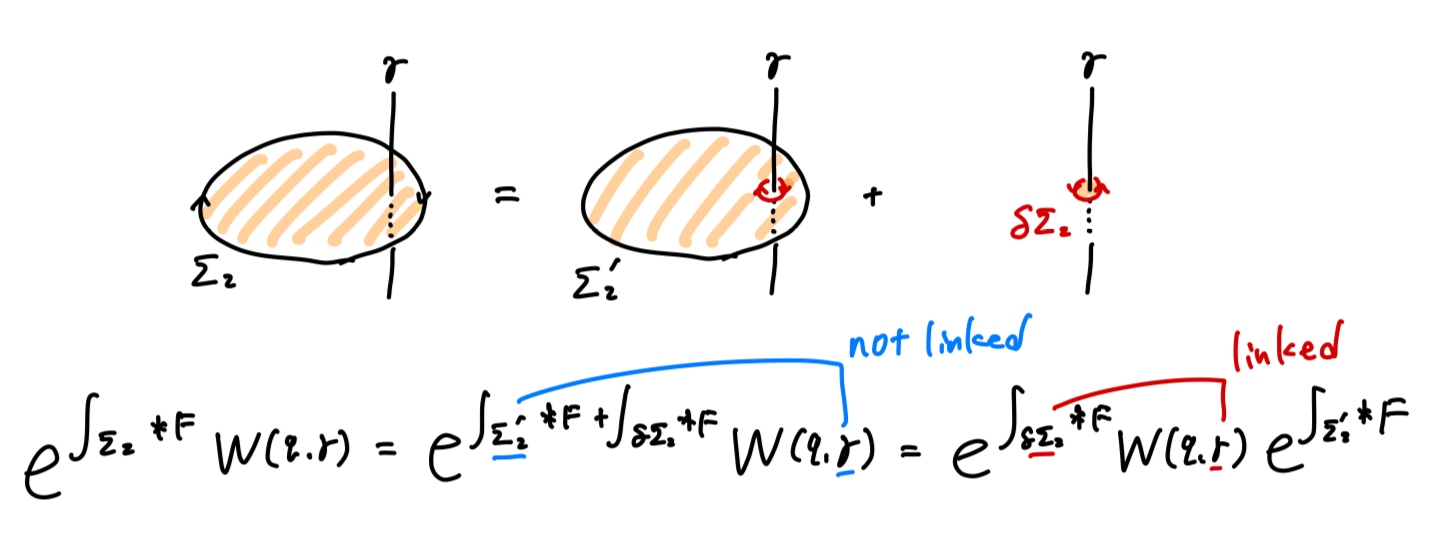
\includegraphics[width=0.8\textwidth]{ActionToWilsonLine.jpg}
    \caption{$\Sigma_2=\Sigma'_2\cup \delta \Sigma_2$, where $\Sigma_2$ is a boundary of infinitesimal $3$-dim mfd which links to $\gamma$. }
    \label{ActionToWlison}
\end{figure}
\noindent
Note that this deformation should be interpreted in path-integral formulation
\footnote{This means that we consider Ward-Takahashi identity as the current conservation, rather than Noether's theorem. 
In other words, we consider QFT rather than classical field theory. }
. Thus, we have 
\begin{align}
    \lr{\exp\blr{i\frac{\lambda}{g^2}\oint_{\Sigma_2}\star F}W(q, \gamma)}
    =\lr{e^{iq\lambda\mathrm{Link}(\Sigma_2, \gamma)}
    W(q, \gamma)\exp\blr{i\frac{\lambda}{g^2}\oint_{\Sigma'_2}\star F}W(q, \gamma)}, 
\label{WlisonLineCharge}
\end{align}
which is the same as \eqref{ActionWilson}. \\
 By the way, the action of $U^e_\lambda$ on $W(q, \gamma)$ can be seen as the shift of 1-form gauge field $A$ by 
 $A\mapsto A + a$, where $\oint_{\gamma} a =\lambda \mathrm{Link}(\Sigma_2, \gamma)$. 
 In fact, the associate current $\star J^e$ is the conjugate momentum of $A$, generating the shift of $A$. \\
 \\
  We can also consider the "dual" $1$-form symmetry: due to the Bianchi identity, we have $dF=0$ (that is, the pure Maxwell field is flat). 
 By regarding this identity as the conservation of $2$-form current $J^{m}_2 :=\frac{1}{2\pi}\star F$, we can write down the correponding symmetry operator as
 \begin{align}
    U^{m}_\lambda(\Sigma_2) = \exp\blr{i\lambda\oint_{\Sigma_2}\star J^m_2}
    =\exp\blr{i\lambda\oint_{\Sigma_2}\frac{F}{2\pi}}. 
 \label{magnetic1form}
 \end{align}
 This $1$-form symmetry is called \textit{magnetic $1$-form symmetry}. Its charged operator is the so-called \textbf{'t Hooft line}
 \begin{align}
    T_1(m, \gamma) := e^{im\int_{\gamma}\tilde{A}}, 
 \label{tHooft}
 \end{align}
 where $\tilde{A}$ is the dual gauge field defined by $\star F=d\tilde{A}$. 
 The action of the $1$-form magnetic symmetry on a 't Hooft line is completely analogous to the case of electric $1$-form symmetry: 
 \begin{align}
    \lr{U^{m}_\lambda(\Sigma_2)T_1(m, \gamma)}
    =e^{im\lambda\mathrm{Link}(\Sigma_2, \gamma)}\lr{T_1(m, \gamma)U^{m}_\lambda (\Sigma'_2)}. 
 \label{ActionTotHooft}
 \end{align}
 \subsubsection{Gauging $1$-form $U(1)$ symmetry}
 It is insightful to consider coupling "background gauge field" to our conserved $2$-form currents, as we have done in the case of ordinary $U(1)$ gauge theory. 
This is done by adding to the action integral
\footnote{詮: 系の力学を記述する「作用積分」と, 演算子の場に対する「作用」を区別するために, 以降は(文脈から明らかな場合を除いて)前者を"action integral"と呼ぶことにします. }
 the term $\int B^e_2\wedge \star J^e_2$ and $\int B^m_2\wedge \star J^m_2$ respectively, 
where $B^e_2$ and $B^m_2$ are the $2$-form background gauge field of $1$-form electric/magnetic symmetry.  
The modified action integral would be of the form 
\begin{align}
    S_1=\frac{1}{2g^2}\int (F-B^e_2)\wedge \star (F-B^e_2) 
    +\frac{i}{2\pi}\int B^m_2 \wedge F
    =\frac{1}{2g^2}\int F\wedge \star F -\frac{1}{g^2} B^2 \wedge F
    +\frac{1}{2g^2}\int B^e_2\wedge B^e_2 + 
    \frac{i}{2\pi}\int B^m_2\wedge F. 
\label{Gauging1formSym}
\end{align}
The new term $\int B^e_2\wedge B^e_2$ is to ensure the invariance of the kinetic term $\int F\wedge \star F$
under the gauge transformation $A\to A+ \lambda^e_1,~ B^e_{2}\to B^e_2 + d\lambda^e_1$ ($\lambda^e_1$ : some (non-closed) $1$-form). 
Note that, this term does not affect the dynamics of the theory unless we treat $B^e_2$ and $B^m_2$ just as "background" fields 
(so, the choice of such an additional term is not unique: we will point out that again below). 
This action is invariant under magnetic $1$-form transformation $\tilde{A} \to \tilde{A}+\lambda^{m}_1, ~B^m_2\to B^m_2 + d\lambda^m_1$, 
but not invariant under electric $1$-form transformation $A\to A+ \lambda^e_1,~ B^e_{2}\to B^e_2 + d\lambda^e_1$: 
\begin{align}
    \delta S_1 = \frac{i}{2\pi}\int B^m_2\wedge d\lambda^e_1. 
    \label{eleAno}
\end{align}
Thus, the magnetic $1$-form symmetry can be gauged consistently under this $S_1$ while the electric $1$-form cannot. \\
 Another choice of modification might be
\begin{align}
    S_2 = -\frac{1}{2g^2}\int (F-B^e_2)\wedge \star (F-B^e_2)
    +\frac{i}{2\pi}\int B^m_2\wedge(F-B^e_2), 
\end{align}
The action is in turn invariant under electrum $1$-form symmetry, 
but not under the magnetic $1$-form transforastion $
A^m\to A^m + \lambda^m_1, ~B^m_2\to B^m_2 + d\lambda^m_1$ : 
\begin{align}
    \delta S_2 = \frac{i}{2\pi}\int -d\lambda^m_1\wedge B^e_2. 
    \label{magAno}
\end{align}
Combining the two observation, we can see that 
we cannot make both electric and magnetic $U(1)$ $1$-form symmetry simultaneous by any choice of additionallocal term. 
Such a situation is described that the action of $3+1$-d Maxwell theory has a mixed 't Hooft anomaly of $U(1)^{(1)}_e$, $U(1)^{(1)}_m$. \\
 Let us see the mixed anomaly \eqref{magAno} from the inflow pitcure briefly. 
We consider the following "anomaly inflow action" in five dimension: 
\begin{align}
    S_{\mathrm{inflow}} = -\frac{i}{2\pi}\int_{N_{5}} B^{m}_2\wedge dB^e_2, 
\end{align}
where $\partial N_5 = M_4$ is our spacetime manifold. By the background gauge transformation $B^m_2 \to B^m_2 + d \lambda^m_1$, we have
\begin{align}
    \delta S_{\mathrm{inflow}} &= -\frac{i}{2\pi}\int_{N_5} d\lambda^m_1 \wedge dB^e_2 \\
    &=-\frac{i}{2\pi}\int_{N_5}\blr{d(d\lambda^m_1\wedge B^e_2)-d^2\lambda^m_1 \wedge dB^e_2}\\
    &=-\frac{i}{2\pi}\int_{\partial N_5}d\lambda^m_1\wedge B^e_2 + 0~~
    (\because \mathrm{Stokes' thm})\\
    &=-\frac{i}{2\pi}\int_{M_4}d\lambda^m_1\wedge B^e_2, 
\end{align}
which is just the same as $\delta S_2$ in \eqref{magAno}. 
Therefore, we can add $-S_{\mathrm{inflow}}$ in our action integral to cancel the mixed 't Hooft anomaly 
in the boundary $M_4$. 
%%%%
%%%%
\subsubsection{Electric-magnetic duality}
This part is mainly based on \cite{TD}. Please see his video for detail. \\
 Let's now consider the following action integral, whose dynamical gauge field is $\tilde{A}$:
\begin{align}
    S[\tilde{A}, F]
    =-\frac{1}{2g^2}\int F\wedge \star F + \frac{i}{2\pi}\int d\tilde{A}\wedge F. 
\label{dualityAction}
\end{align}
The action is the form of coupling magnetic $2$-form current $\star J^{m}_2 = \frac{1}{2\pi}F$ to dynamical gauge field $\tilde{A}$. 
"Integraling out" the $\tilde{A}$ field obviously reproduces the action \eqref{U1pure}, 
which means that 
gauging magnetic $1$-form symmetry $U^{(1)}_m$ yields an electric $1$-form symmetry $U^{(1)}_e$. \\
 Another way to study the relation of $U^{(1)}_e$ and $U^{(1)}_m$ is to consider the equation of motion for $\tilde{A}$ in the action \eqref{dualityAction}, 
which is
\begin{align}
    \frac{i}{g^2}\star F = -\frac{1}{2\pi}d\tilde{A} \ler{=: \frac{1}{2\pi}\tilde{F}}. 
\end{align}
By using the property of Hodge star operator for arbitrary $p$-form $\omega$, 
$\star\star \omega = (-1)^{p(d+1-p)}\omega$ (for our case $p=2$), we can also have
\begin{align}
    \star \tilde{F}= -\frac{2\pi i}{g^2}F. 
\end{align}
Then we can rewrite the action \eqref{dualityAction} using $\tilde{A}$ only: 
\begin{align}
    \tilde{S}[\tilde{A}]
    &=-\frac{1}{2g^2}\int \ler{\frac{g^2}{2\pi i}\star \tilde{F}}\wedge \ler{\frac{g^2}{2\pi i}\tilde{F}} + \frac{i}{2\pi}\int \tilde{F}\wedge \ler{\frac{g^2}{2\pi i}\star \tilde{F}}\\
    &=-\frac{g^2}{8\pi^2}\int \tilde{F}\wedge \star \tilde{F}. 
\end{align}
Then, this $\tilde{S}[\tilde{A}]$ becomes the same form of the original action under the EoM of dynamic field $\tilde{A}$. 
But the coupling constant is different: for the theory of $\tilde{S}$, 
\begin{align}
    \frac{1}{2\tilde{g}^2} = \frac{g^2}{8\pi^2} ~\to~\tilde{g}^2 = 4\pi^2 / g^2.  
\end{align}
This means that, when the original coupling constant of the original dynamical field $A$ becomes smaller, 
the "dual" coupling constant of the dual field $\tilde{A}$ becomes larger. \\
 This duality picture gives us an important viewpoint of the symmetry: 
symmetry operators act on defect operators, which generates the symmetry of the system. 
In other words, the algebra of symmetry operators is the representation of the symmetry, 
whose representation space is spanned by defect operators. 
Generally, this algebraic structure is not necessarily group-like 
(called "higher group"), 
so we will go on a journey to the representation theory of category (圏) 
in order to study the physics under generalized symmetry. 
%
%
%
%
%
\newpage
\section{A brief intro to Non-invertible symmetry}
%ここからは, 先に述べた「2つの一般化の方向」の, もう一つに視点を当ててみる. 
%今までの議論において, 対称性演算子には常にその逆元が存在していた. 
%いま, そのような制約を緩めた時にどのような「対称性」が現れるのかを考える. 
%これはもはや通常のgroup-likeな対称性ではなく, 「非可逆対称性」あるいは"non-invertible symmetry"と呼ばれるものになる. \\
%非可逆的対称性の持つ代数構造は群をなさないが, それはフュージョン圏と呼ばれる圏の構造を有している. 
%もう少しだけ言うと,非可逆対称性を持つ理論において, そこに現れるsymmetry defect operatorたちの間には"fusion rule"という関係があり, 
%これはdefect同士を"fuse"して別のdefectを生み出すという点で, defectとdefectの間の射であるとみなせる. 
%すると, (simple) defectを対象, defect同士の変換則=fusion ruleを射とした圏を考えることができるが, 
%この圏にはテンソル積および"F-symbol"という自然変換が備わっているという点で, 
%一般の圏よりも代数的に「豊かな構造を持っている」圏(=フュージョン圏)をなすということがわかる. \\
Let us now turn our attention to the other of the “two generalization directions” mentioned earlier. 
In the previous discussions, symmetry operators have always had their inverses. 
Now, let us consider what kind of “symmetry” will appear when such restrictions are relaxed. 
This is no longer the usual group-like symmetry, but is what we call "non-invertible symmetry" or "non-invertible symmetry". \\
\\
 We start from the very abstract point: the algebra of such a new symmetry. 
\subsection{Algebraic structure of Non-invertible symmetry: fusion category}
\noindent
\tiny
(This part is never mathematically rigorous. I guess Yao is a lot more familiar with these topics. 
I mainly referred to \cite{KI} when writing this part)\\
\normalsize
 The algebraic structure of non-invertible symmetry is not a group, but it in general has a categorical structure called "fusion category". 
To say more, in a theory with non-invertible symmetries, there is still a "fusion rule" relation among symmetry defect operators in the theory. 
This is regarded as morphisms among different defects, in the sense that defects "fuse" with each other to create another defect 
(note that, for systems with group-like symmetry, the fusion rule becomes just the group multiplication rule). 
Then, we can consider a category with (simple) defects as "objects" and the fusion rule between defects as "morphisms". 
Such type of categories are what we call \textit{fusion category}. \\
% This category has a "richer structure" algebraically than the general category, 
%in that it has a tensor product and a natural transformation called "F-symbol". (=fusion sphere) in that this sphere has tensor products and “F-symbol” natural transformations. 
\\
 A (unitary) fusion category $\mathcal{C}$ is a category which consists of the following information:
\begin{itemize}
    \item Objects $x, y, \cdots \in \mathcal{C}$, including a unit object $1\in \mathcal{C}$. 
    \item Morphisms $\mathrm{Hom}(x,y)$: a finite dimensional $\cpl$-vector space, 
    equipped with an adjoint $\dagger: f\in \mathrm{Hom}(x,y)\mapsto f^\dagger \mathrm{Hom}(y,x)$. 
    \item Bifuncters $\otimes: \mathcal{C}\times \mathcal{C}\to \mathcal{C}$ (tensor product), $\oplus: \mathcal{C}\times \mathcal{C}\to \mathcal{C}$ (direct sum).  
    \item Natural isomorphisms $\alpha_{x,y,z}: (x\otimes y)\otimes z\to x\otimes (y\otimes z)$ (associator), $l_x: 1\otimes x\to x$ (left unit), $r_x: x\otimes 1\to x$ (right unit). 
    These satisfy certain conditions (shown later). These isomorphisms are also unitary with respect to the adjoint $\dagger$. 
\end{itemize}
 An object $x\in \mathcal{C}$ is called simple when it cannot be decomposed into a direct sum of objects. 
The important property of fusion category is that, 
there is only finite number of simple objects (up to isomorphism), and 
every object is isomorphic to a direct sum of finitely many simple objects: 
$x\simeq \bigoplus_{i}N_i a_i$ where $\{a_i\}$ is a set of simple objects and $N_i$ is a non-negative integer. 
In application to physics, we can exploit this property to discuss the "fusion rule" of topological operators. \\
 Another important property is the existence of dual object $x^*$ for every $x\in \mathcal{C}$. 
The "duality" is in the sense that there are a pair of morphisms 
$\mathrm{ev}^{L}_x: x^*\otimes x \to 1$ (evaluation) and $\mathrm{coev}^{L}_x: 1\to x\otimes x^*$ (coevaluation) which satisfies the following relations: 
\begin{align}
    &r_x\circ (id_x\otimes \mathrm{ev}^L_x)\circ \alpha_{x, x^*, x}\circ (\mathrm{coev}^L_x\otimes id_x)\circ l^{-1}_x = id_x, \\
    &l_{x^*}\circ(\mathrm{ev}^L_x\otimes id_{x^{*}}) \circ \alpha^{-1}_{x^*, x, x^*}\circ (id_x^*\otimes \mathrm{coev}^{L}_x)\circ r^{-1}_{x^*}=id_{x^*}. 
    \label{eval}
\end{align}
These morphisms are not unitary in general
\footnote{Are there any condition when those morphisms become unitary? }
The adjoints $\mathrm{ev}^R_x = (\mathrm{ev}^{L}_x)^\dagger$ and $\mathrm{coev}^{R}_x = (\mathrm{coev}^{L}_x)^\dagger$ 
 The associavity and left/right units satisfy the following identity, written in a language of commutative diagram: 
\begin{figure}[H]
    \centering
    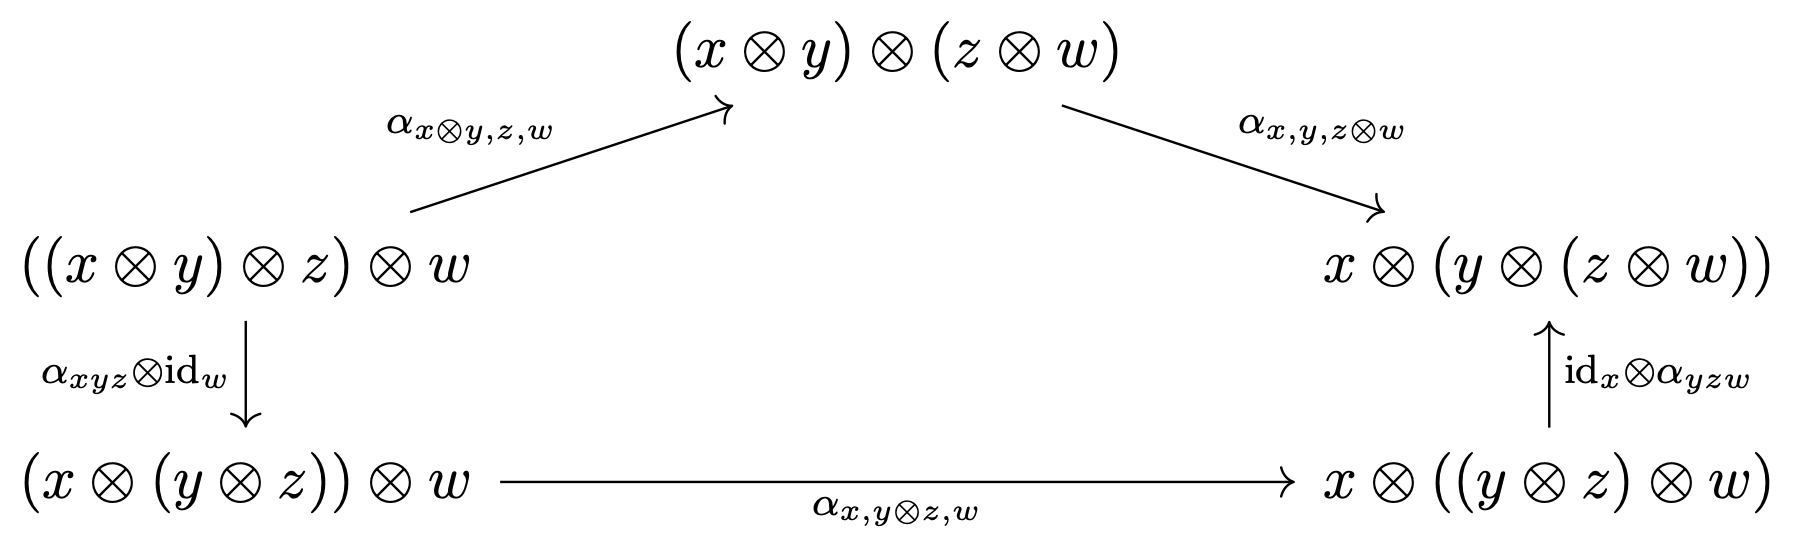
\includegraphics[width=0.7\textwidth]{pentagon.png}
    \caption{The "pentagon identity" of the associator $\alpha_{x,y,z}$, for $x,y,z\in \mathrm{Obj}(\mathcal{C})$. 
    Images from \cite{KI}. }
    \label{pentagon}
\end{figure}
\begin{figure}[H]
    \centering
    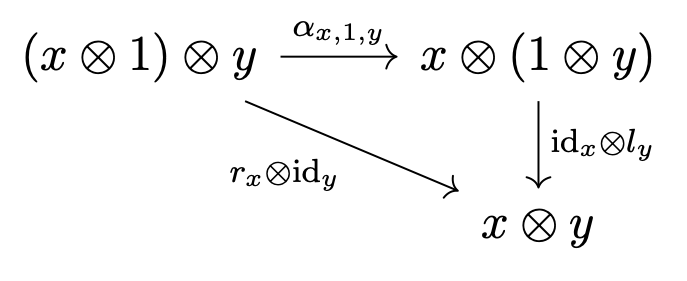
\includegraphics[width=0.7\textwidth]{lrunits.png}
    \caption{The identity of left and right units. 
    Images from \cite{KI}. }
    \label{lrunits}
\end{figure}
%\begin{itemize}
 %   \item tensor functor
  %  \item natural transformation 
%\end{itemize}
  Informally speaking, the algebraic structure of non-invertible symmetry cannot be totally arbitrary: 
  there should be some rules. 
  More precisely, we need some "consistency condition" for creating physically valid models, 
  although this is not as strict as group-like. 
  Such a rule is the pentagon identity of the associavity transformation 
  $\alpha_{x,y,z}: (x\otimes y)\times z\mapsto x\times (y\times z)$ mentioned above \ref{pentagon}. \\
   A practically important point is that, the pentagon identity enables us to write down the general form of the fusion rule, given by the coefficients called "F-symbol": 
  \begin{figure}[H]
    \centering
    \resizebox{0.6\textwidth}{!}{%
    \begin{circuitikz}
    \tikzstyle{every node}=[font=\LARGE]
    \draw [line width=0.9pt, short] (5,7.75) -- (5,4);
    \draw [line width=0.9pt, short] (5,7.75) -- (2.5,11.5);
    \draw [line width=0.9pt, short] (5,7.75) -- (7.5,11.5);
    \draw [line width=0.9pt, short] (3.75,9.75) -- (5,11.5);
    \draw [line width=0.9pt, short] (15,7.75) -- (15,4);
    \draw [line width=0.9pt, short] (15,7.75) -- (12.5,11.5);
    \draw [line width=0.9pt, short] (15,7.75) -- (17.5,11.5);
    \draw [line width=0.9pt, short] (16.25,9.75) -- (15,11.5);
    \node [font=\LARGE] at (8.75,7.75) {$=$};
    \node [font=\LARGE] at (9.5,7.75) {$\sum_{b}$};
    \node [font=\LARGE] at (11,7.75) {$[F^{4}_{123}]_{ab}$};
    \node [font=\LARGE] at (5,3.5) {$4$};
    \node [font=\LARGE] at (2.5,12) {$1$};
    \node [font=\LARGE] at (5.25,12) {$2$};
    \node [font=\LARGE] at (7.5,12) {$3$};
    \node [font=\LARGE] at (17.5,12) {$3$};
    \node [font=\LARGE] at (15,12) {$2$};
    \node [font=\LARGE] at (12.5,12) {$1$};
    \node [font=\LARGE] at (15,3.5) {$4$};
    \draw [ color={rgb,255:red,255; green,38; blue,0}, line width=0.9pt, short] (5,7.75) -- (3.75,9.75);
    \node [font=\LARGE] at (5,10) {};
    \draw [ color={rgb,255:red,255; green,38; blue,0}, line width=0.9pt, short] (15,7.75) -- (16.25,9.75);
    \draw [->, >=Stealth] (5,5.5) -- (5,5.75);
    \draw [->, >=Stealth] (15,5.5) -- (15,5.75);
    \draw [->, >=Stealth] (3.25,10.5) -- (3,10.75);
    \draw [->, >=Stealth] (4.25,10.5) -- (4.5,10.75);
    \draw [->, >=Stealth] (4.5,8.5) -- (4.25,9);
    \draw [->, >=Stealth] (14,9.25) -- (13.75,9.75);
    \draw [->, >=Stealth] (15.75,10.5) -- (15.5,10.75);
    \draw [->, >=Stealth] (16.75,10.5) -- (17,10.75);
    \draw [->, >=Stealth] (15.5,8.5) -- (15.75,9);
    \draw [->, >=Stealth] (6,9.25) -- (6.25,9.5);
    \node [font=\LARGE] at (3.75,8.75) {$a$};
    \node [font=\LARGE] at (16.25,8.75) {$b$};
    \end{circuitikz}
    }%
    \label{F-symbol}
    \end{figure}
  Note that the matrix $F_{4}^{123}$ of coefficients is just the identity for the case of group-like symmetry. 
  \\\\
   In a sense, fusion category can be regardeda as a generalization of the category of
  the irreducible representations (irreps.) of a certain finite group $G$ 
  into that of a more general algebraic structure
  \footnote{This algebraic structure is the so-called \textit{Hopf algebra}, 
  which can be undeestood as an abstraction of group property. 
  Hopf algebra is }
  . 
  In other words, the category of irreps. of finite group $\mathrm{Rep}(G)$ is one simple example of fusion category. 
  This consists of 
  \begin{itemize}
    \item Objects: (unitary equivalence class of) irreps. of a finite group $G$, including the trivial rep. as the unit object. 
    \item Morphisms: $\mathrm{Hom}(\pi, \sigma) = \blr{T|T\pi(g) = \sigma(g)T, ~\forall g\in G}$ 
    (the set of linear maps from one representation space to another: $V_\pi\to V_\sigma$, called "intertwiner"). 
    \item Bifunctors: tensor products (here it is just associative: $\pi\times \sigma \simeq \sigma\times \pi$), direct sum. 
  \end{itemize}
  The fusion rule here is nothing but the direct sum decomposition (block diagonalization) of the tensor product of two irreps. 
  (up to constant coefficient): 
  \begin{align}
    \pi \otimes \sigma \simeq \bigoplus_i n_i \rho_i, 
  \end{align}
  where $n_i$s are non-negative integers. 
  We may have encountered this kind of fusion in the case of $SU(2)$: 
  in that case, we have succeeded in writing down the exact coefficients as 
  Clebsh-Gordan coefficients. \\
 We may notice that this does not form a group (there is no "inverse" of representation). 
Still, we have a "dual" $\pi^*$ for each irrep. $\pi$, whose duality is characterized by the fact that
 the decomposition of the tensor of a given irrep. $\pi$ and its dual includes the trivial rep. : 
 \begin{align}
    \pi\otimes \pi^* \sim 1\oplus \cdots. 
 \end{align}
 The right side does not need to be equal to $1$. 
  \\
   There is another thing: for each object in $\mathrm{Rep}(G)$, we can assign a natural number called "dimension", satisfying
  \begin{align}
    \dim{(\pi \otimes \sigma)} &= (\dim(\pi))(\dim(\sigma)), \\
    \dim(\bigoplus_i \pi_i) &= \sum_i \dim{\pi_i}. \\
  \label{dim}
  \end{align}
  You may notice that this $\dim$ is just the rank of representation matrices. 
  In fact, the concept of $\dim$ can also be extended to a general fusion category symmetry. 
  However, in most general case, this $\dim$ is not necessarily a natural number: still it can be non-negative real number. 
  In physics, such a number is called "quantum dimension" of topological operators. 
  \\
  \\
   In short, there are two messages to take home: 
  \begin{itemize}
    \item The algebraic structure of non-invertible symmetry is in general given by a category, which is "weaker" than group. 
    \item However, it is not an arbitrary category. Rather, it must be a fusion category:
     it has a finite number of objects on which we can perform the "fusion rule", tensor product with associativity, and some other special properties. 
  \end{itemize}
Therefore, when we encounter physical systems which supports non-invertible symmetry, 
we can find the hidden categorical structure, and study the physical property of systems by exploiting the algebraic property of fusion category. 
There are also "inverse" attempts: to a given fusion category, we may succeed in providing the proper theory (TQFT) which encodes the categorical structure. 
Many works have been done on such attempts, especially for lattice field theory. 
\subsubsection{Relation to anyon statistics in $1+1$d: \textit{braiding}}
\color{red}
Undone
\color{black}

From the perspective of categorical symmetry, 
the symmetry structure of anyon is given as a \textit{braiding} on a monoidal category, 
which is a natural isomorphism $c_{X,Y}: X\otimes Y \to Y\otimes X$
 that satisfies the "hexagon identity" (hexagonal diagram): 
 \begin{figure}[H]
    \centering
    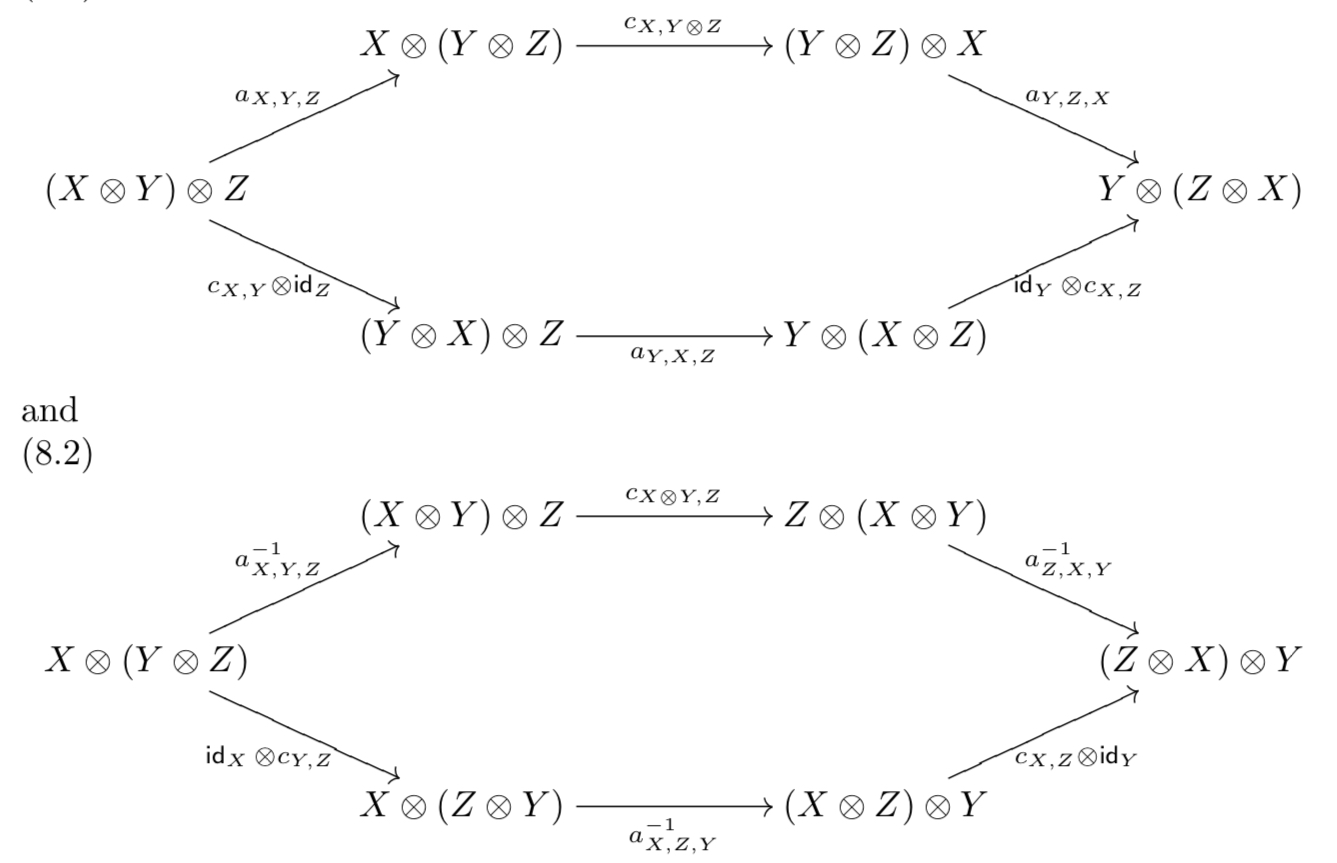
\includegraphics[width=0.6\textwidth]{hexagon.jpeg}
    \caption{The "hexagon identity" of braiding $c_{X,Y}: X\otimes Y \to Y\otimes X$. 
    Images from \cite{PESGDNVO}. }
    \label{lrunits}
\end{figure}
\subsection{Example from lattice: $1+1$-d Ising CFT}
The (probably) most typical example of field theory with non-invertible symmetry is 
of the critical transverse-field Ising model (TFIM). Its Hamiltonian is given by
\begin{align}
    H = -\sum_{j=1}^{L}(Z_{j-1}Z_j + X_j), 
\end{align}
with periodic boundary condition $X_j = X_{j+L}, Z_j=Z_{j+L}$. \\
 This model has $\zet_2$ symmetry $X_i\mapsto -X_i, ~Z_i\mapsto -Z_i$. 
The symmetry operator of this $\zet_2$ is the identity $1$ and
\begin{align}
    \eta = \prod_{j=1}^{L}X_j.  
\end{align}
We can easily check that $\eta^\dagger=\eta$ and $\eta^2=1$. 
This means that the set of unitary operators $\{1, \eta\}$ generates the $\zet_2$ action on the Hilbert space $\mathcal{H}$. \\
 In addition, this is also invariant under the following "Kramers-Wannier transformation": 
\begin{align}
\label{KW}
X_j\mapsto Z_{j-1}Z_j, ~~ Z_{j-1}Z_j \mapsto X_{j-1}. 
\end{align}
We will see that this is indeed non-invertible. First, we can check that
\begin{align}
    (X_j, Z_{j-1}Z_j)\mapsto (Z_{j-1}Z_j, X_{j-1})\mapsto (X_{j-1}, Z_{j-2}Z_{j-1}). 
\end{align}
This means that performing the KW transformation twice is equivalent to the shift (lattice translation) by one site. 
Sometimes, KW transformation on lattice is called "non-invertible lattice translation" (see, for example, \cite{NSSSSHS}). 
Second, it can be shown that this KW cannot be represented by any unitary operator. 
In fact, if there were such a unitary operator $U_{KW}$, 
we would act it on $\eta$ to obtain
\begin{align}
    U_{KW}\eta U^{-1}_{KW} = U_{KW} \prod_{j=1}^{L} X_j U^{-1}_{KW}
    =\prod_{j=1}^{L}(Z_{j-1}Z_j) = 1, 
\end{align}
which means $\eta = U^{-1}_{KW}U_{KW}=1$. 
Therefore, the KW transformation cannot be implemented by any unitary (invertible) operator. \\
\\
 Below, we denote the operator generating the KW by $D$. 
The algebraic structure of operators $1, \eta, D$ and the "lattice translation operator" $T$ (re-writing site indices by $i\mapsto i+1$) is, 
to show without derivation, 
\begin{align}
    \eta^2=1, ~\eta T = T \eta, ~\eta D = D \eta = D, ~ DT^{-1} = T^{-1}D = D^\dagger, ~
    D^2 = (1+\eta)T. 
    \label{IsingSym}
\end{align}
We can see that the $D$ is non-invertible since $D$ has no inverse, contrary to $\eta$. 
\\
 Symmetry operators can extend over any closed 1-dimensional loop in 1+1-d spacetime. 
In particular, we can consider symmetry operators extending horizontally in time direction. 
This is the situation where we can see a point-like operator in the exactly same spatial point at any time slice, 
which looks like a "defect" in the Hilbert space. 
We sometimes call such a configuration of topological operator (defect operator) as "twist" of Hilbert space by defect operator. 
In the case of $1+1$-d CFT on torus, we have the invariance under a coordinate transformation called "modular transformation", 
generated by $T: z\to z + 1$ and $S: z\mapsto -\frac{1}{z}$. 
\begin{figure}[H]
    \centering
    \resizebox{0.6\textwidth}{!}{%
    \begin{circuitikz}
    \tikzstyle{every node}=[font=\LARGE]
    \draw [ line width=0.9pt ] (2.5,15) rectangle (10,7.5);
    \draw [line width=0.9pt, ->, >=Stealth] (1.25,6.25) -- (1.25,8.75);
    \draw [line width=0.9pt, ->, >=Stealth] (1.25,6.25) -- (3.75,6.25);
    \draw [ color={rgb,255:red,255; green,38; blue,0}, line width=0.9pt, short] (2.5,11.25) -- (10,11.25);
    \draw [ line width=0.9pt ] (16.25,15) rectangle (23.75,7.5);
    \draw [line width=0.9pt, ->, >=Stealth] (15,6.25) -- (15,8.75);
    \draw [line width=0.9pt, ->, >=Stealth] (15,6.25) -- (17.5,6.25);
    \draw [ color={rgb,255:red,255; green,38; blue,0}, line width=0.9pt, short] (20,7.5) -- (20,15);
    \node [font=\LARGE] at (4.25,6.25) {$x$};
    \node [font=\LARGE] at (1.25,9.25) {$\tau$};
    \node [font=\LARGE] at (18,6.25) {$x$};
    \node [font=\LARGE] at (15,9.25) {$\tau$};
    \draw [line width=0.9pt, ->, >=Stealth] (6,7.5) -- (6.25,7.5);
    \draw [line width=0.9pt, ->, >=Stealth] (4.25,15) -- (6.25,15);
    \end{circuitikz}
    }
    \caption{Modular transformation maps an operator (global on a certain time slice) to a defect (localized on every time slice). }
    \label{SymmetryAndDefect}
    \end{figure}
Now, let's consider to insert a "defect" into our Hilbert space. 
\subsection{Example from continuous: $3+1$-d $U(1)$ Maxwell theory (, again)}
We can also find examples of non-invertible symmetry in continuous QFT. 
Let's consider the action integral
\newpage
\section{What comes next?}
In this section, we will see what comes as following topics after studying gerenalized symmetry in this text. 
I appologize that I do not understand the following topics and cannot explain any details. 
\subsection{Generalized charges}
\subsection{Symmetry TFT}
\newpage
\section{preliminaries}
この分野を勉強するにあたって役に立ちそうな知識を, ごくごく簡単にまとめます. 
higher-form symmetryとその例を理解するにはゲージ理論の知識が, およびnon-invertible symmetryの例を理解するにはCFTの知識が多少必要になります. 
また, 一般の多様体上で微分や積分を局所座標に依存しない形で定式化するためには, 微分形式の言葉が必要になります. 
\subsection{微分形式}
ここでは, 時空多様体$M$は微分可能であり, 局所座標系$\{(U, \phi)\}$($\phi: U\to \re^{d}$)が与えられているものとします. 
そのため, あらかじめ局所表示されたものとして微分形式を取り扱います. 
\subsubsection{$1$-formの導入: 2次元平面を例に}
いま, 2次元平面$M=\re^{2}$の上の各点$(x,y)$ごとにベクトル$(a_x(x,y), a_y(x,y))$が定義されている, つまりベクトル場が定まっているとする. 
このベクトル場を, $M$上の曲線$\gamma: [0,1]\to M, ~ t\mapsto (x(t), y(t))$に沿って積分したい. 
\begin{align}
    \begin{tikzpicture}
        \draw (-2,-2)--(2,-2)--(2,2)--(-2,2)--(-2,-2);
        \draw[->] (-1,-1) .. controls (-0.5, -1.2) and (0.5,1.2) .. (1,1);
        \node[above] at (0,0) {(x(t), y(t))};
        \node[above] at (-0.5,-0.5) {\gamma};
        \fill[black](0,0) circle [radius=0.05];
    \end{tikzpicture}
\end{align}
この積分は, 
\begin{align}
    \int_{0}^{1} \left(a_x(x(t), y(t))\frac{dx}{dt}dt + a_y(x(t), y(t))\frac{dy}{dt}dt \right)
    \equiv \int_{\gamma} a_x dx + a_y dy
\end{align}
と書ける. 
点$p=(x,y)\in M$に対して, $\ler{\frac{\partial}{\partial x}}_p : C^{\infty}(M)\to \mathbb{R}, f\to \frac{\partial f}{\partial x}(x,y)$および
$\ler{\frac{\partial}{\partial y}}_p : f\to \frac{\partial f}{\partial y}(x,y)$
という2つの写像を定める時, 基底$\blr{\ler{\frac{\partial}{\partial x}}_p, \ler{\frac{\partial}{\partial y}}_p}$で張られる線型空間$T_pM$は$M$の点$p$における接空間と呼ばれ, 
$T_pM$の元は接ベクトルと呼ばれる. 接ベクトルは時空座標の軌跡の情報を持つ. \\
 いま, 接空間の双対空間$T^{*}_pM$, すなわち$\phi: v\in T_p M \mapsto \phi(v)\in \mathbb{K}$ によって張られる線型空間を考える
(係数体$\mathbb{K}$はなんでも良いが, 以下では$\mathbb{R}$とする). 
$T^{*}_pM$の基底を$\blr{dx_p, dy_p}$と書き, これを
双線型写像$\langle \rangle: T_pM \times T^{*}_pM \to \re$によって
\begin{align}
   & \langle \ler{\frac{\partial}{\partial x}}_p, dx_p \rangle = 1,~~ \langle \ler{\frac{\partial}{\partial y}}_p, dx_p \rangle = 0\\
    &\langle \ler{\frac{\partial}{\partial x}}_p, dx_p \rangle = 1,~~ \langle \ler{\frac{\partial}{\partial y}}_p, dy_p \rangle = 1
\end{align}
となるものとする. この時, $dx$および$dy$を, 「各点$p=(x,y)\in M$ごとに, 余接空間$T_p M$の基底$\blr{dx_p, dy_p}$を与えるもの」として, 
$\omega\in \Omega^{1}(M): M\to T^{*}M$を「各点$p=(x,y)$ごとに余接ベクトル$\omega_x(x, y)dx_p + \omega_y(x,y)dy_p$を与えるもの」とする. 
このような$\omega$を$M$上の$1$-formと呼ぶ. 
集合$\Omega^{1}(M)$は, $dx$および$dy$の$C^{\infty}(M)$係数線型結合($C^{\infty}$-加群)の構造を有する. \\
 $1$-formは, 各点における接ベクトルを与えるごとに数を返すため, 「経路$\gamma$に沿った$1$-formの積分」を定義できる: 
\begin{align}
    \int_{\gamma} \omega
    =\int_{0}^{1} \left(\omega_x(x(t), y(t))\frac{dx}{dt}dt + \omega_y(x(t), y(t))\frac{dy}{dt}dt \right)~.
\end{align}
すなわち, $1$-form$\omega_x(x, y)dx_p + \omega_y(x, y)dy_p$の積分は, 接ベクトル$\omega_x(x, y)\ler{\frac{\partial}{\partial x}}_p + \omega_y(x,y)\ler{\frac{\partial}{\partial y}}_p$の積分と結局同じである. \\
 $dx_p$および$dy_p$を点$p=(x,y)$における線素とみなせば, $\omega_p = \omega_x(x,y)dx_p + \omega_y(x,y)dy_p$を, 単に「軌跡$\gamma$に沿った関数の微小変化」と考えることもできる. 
実際, ある関数$f: M\to \re$を用いて$\omega_x(x,y)=\partial_x f(x,y)$, $\omega_y(x,y) = \partial_y f(x,y)$と書ける時, 
$\omega_p = \partial_x f(x,y) dx_p + \partial_y f(x,y) dy_p$で, これはまさに関数$f$の点$p$における微小変化の形. 
\subsubsection{微分形式の定義}
一般の$n$次元可微分多様体においても同様に, 各点$p\in M$の接空間$T_pM$に対する双対空間(余接空間)を考える事で, 
$1$-form $\omega\in \Omega^{1}(M)$を定義出来る. 
多様体$M$の局所座標表示$\{U, \phi\}$が与えられているとすると, 各点$p\in U$上での$\omega$の局所表示は, 一般に$\omega=\sum_{\mu}f_{\mu}(x)dx^{\mu}\in \Omega^{1}(M)$の形をとる. 
この時, 2次元平面の場合と同様に, $1$-formの経路$\gamma: [0,1]\to M$に沿った積分というものを考える事ができる(「経路$\gamma$に沿った積分」を, $1$-formに対して数を返す対応と見なす事ができる). 
$1$-formは接ベクトルの"dual"であり, 各点$p\in M$における接ベクトル$v_p=\sum_{\mu}v^{\mu}(x)\ler{\frac{\partial
}{\partial x}}_p$に対して$1$-formを割り当てる写像を, 
\begin{align}
    v_p \mapsto \omega_p = \sum_{\mu\nu}g_{\mu\nu}v^{\nu}(x)dx^{\mu}_p
\end{align}
によって定める事ができる. 
以下, 局所表示の存在を前提として, 特定の点$p\in M$への依存性を明示しないものとする. \\
 $1$-form全体の集合$\Omega^{1}(M)$に対して, 各点ごとに二項演算$\wedge$を定める: 
\begin{align}
    \omega\wedge \eta = \ler{\sum_{\mu}\omega_\mu(x)dx^{\mu}}\ler{\sum_{\nu}\omega_\nu(x)dx^\nu}
    =\sum_{\mu, \nu}\omega_{\mu}(x)\eta_{\nu} dx^{\mu}\wedge dx^{\nu}
\end{align}
これは$\Omega^{1}(M)$の基底の部分について反対称な演算である: $dx^{\mu}\wedge dx^\nu = -dx^\nu \wedge dx^\mu$. 
$1$-form同士のwedge積$\omega\wedge \eta$は, $dx^{\mu}\wedge dx^\nu$の$C^{\infty}(M)$係数線型結合($C^{\infty}(M)$-加群)の形をとる. 
ここで, $M$上の"2-form"全体の集合$\Omega^{2}(M)$を, $\omega_2 = \sum_{i_1, i_2}f_{i_1, i_2}(x)dx^{i_1}\wedge dx^{i_2}$なる形の元によって生成される$C^{\infty}(M)$-加群として定義すると, 
wedge積は2つの1-formに対して2-formを返す反対称な演算であると言える. 
2-formは, 各点$p\in M$において接ベクトル空間の直積$T_pM\times T_p M$を数に移す写像を定める. \\
 より一般に, $M$上の"k-form"全体の集合$\Omega^{k}(M)$を, $\omega_k = \sum_{i_1, \cdots, i_n}f_{i_1, \cdots, i_n}(x)dx^{i_1}\wedge \cdots \wedge dx^{i_n}$なる元により生成される$C^{\infty}(M)$-加群として定義する. 
この時, $p$-formと$q$-formの間のwedge積を, $(p+q)$-formを返す反対称な演算として定義出来る: 
$\alpha_p = \sum_{i_1, \cdots, i_p}\alpha_{i_1, \cdots, i_p}(x)dx^{i_1}\wedge \cdots \wedge dx^{i_p}$
および$\beta_q = \sum_{j_1, \cdots, j_q}\beta_{j_1, \cdots, j_q}(x)dx^{j_1}\wedge \cdots \wedge dx^{j_q}$に対し, 
\begin{align}
    &\alpha_p \wedge \beta_q = \sum_{i_1, \cdots, i_p, j_1, \cdots, j_q}\alpha_{i_1, \cdots, i_p}(x)\beta_{j_1, \cdots, j_q}(x)(dx^{i_1}\wedge \cdots \wedge dx^{i_p})\wedge (dx^{j_1}\wedge \cdots \wedge dx^{j_q}), \\
    &\alpha_p \wedge \beta_q = (-1)^{pq}\beta_q \wedge \alpha_p. \\
\end{align}
このことから, 集合$\Omega^{*}(M):=\bigoplus_{k}\Omega^{k}(M)$を定めた時, これは各$p\in M$ごとに(あるいは, 各開近傍$U\subset M$ごとに)$\mathbb{R}$上の次数付き反可換代数$\Omega^{*}(U)$を定める事がわかる
\footnote{代数構造は大域的には定義されておらず, 各点の近傍$p\in U\subset $にまでしか拡張できない. 
そのため, 微分形式の代数構造に着目する時は, 今後$\Omega^{k}(U)$と書くように努める. }. \\
\subsubsection{外微分}
$d: \Omega^{k}(U)\to \Omega^{k+1}(U)$を, 
\begin{align}
    d\omega 
    = \sum_{h_1\cdots h_p}\sum_{i} \frac{\partial a_{h_1\cdots h_p}}{\partial x_i}dx^{i}\wedge dx^{h_1}\wedge \cdots \wedge dx^{h_p}
\end{align}
\subsubsection{Stokesの定理}
\begin{align}
    \int_{M}d\omega = \int_{\partial M}\omega
\end{align}
\subsubsection{de Rhamコホモロジー}
コホモロジー群というのはホモロジー群
\footnote{位相空間$M$のホモロジー群とは, 簡単に言えば「"境界を取ると消えるもの"と"何らかの境界になっているもの"との間の差を測る指標」であり, 
これは$M$の位相構造に直接的に依存する. 
例えば, ユークリッド空間$\mathbb{R}^n$のような「普通の」空間の中では二者の差はなく(ホモロジー群は自明), トーラス$T^2$では二者は区別される. 
ホモロジー群には様々なバリエーションがあるが, 一番直感的に理解しやすいものは, 三角形分割可能な位相空間に対する単体的ホモロジー
($n$-チェインを$n$-単体の形式和として, 境界準同型を「$n$-単体の図形としての境界を(向きを考慮して)取ってくるもの」として構成するホモロジー)だろう. 
詳しくは, \href{https://ja.wikipedia.org/wiki/単体的ホモロジー}{Wikipediaの記事}を参照. }
の双対(co-)であり(チェイン複体およびその間の境界準同型に対して「転置」を考える事, とも言える), 
「コチェイン複体」と呼ばれる対象および「微分」という操作を用いて構成されるアーベル群の列のことを言う. 
標語的には, これは
「"微分すると0になるもの"と"何らかの微分として書けるもの"との間の差を測る指標」として理解される
\footnote{もちろん(?), コホモロジー理論には公理的な定式化があり, 
"Eilenberg-Steenrod公理"と呼ばれるコホモロジー理論を特徴付ける一連の公理系が存在する: \\
位相空間の組$(X, A\subseteq X)$の圏からアーベル群の圏への反変関手の組$h^{i}$であって, \\
「次元公理(一点空間$X=*$に対して, $h^i(*)=0(i\neq 0), \mathbb{Z}(i=0)$)」\\
「切除公理($U\subseteq A \subseteq X$に対して, 同型$h^{n}(X\backslash U, A\backslash U)\simeq h^n(X, A)$が成り立つ)」\\
「ホモトピー公理(位相空間の組の間のホモトピックな2つの連続写像$f, g$から誘導される群準同型$h^i(f), h^i(g)$は同じ)」\\
「完全性公理(長完全列: $\cdots\to h^i(X, A)\to h^i(X)\to h^i(A)\stackrel{d}{\to}h^{i+1}(X, A)\to\cdots$が成立する)」\\
「加法性公理($(X, A)=(\sqcup_\alpha X_\alpha, \sqcup_{\alpha}A_\alpha)$に対して, 
包含写像$(X_\alpha, A_\alpha)\hookrightarrow (X, A)$は同型$h^i(X, A)\simeq  \prod_{\alpha}h^{i}(X_\alpha, A_\alpha)$を引き起こす)」\\
の5つの性質を満たすものを, コホモロジー理論という. 
詳細を述べる余裕はないので省略. }
. 
コホモロジー群は, コチェイン複体の構成の仕方に応じて様々な種類があるが, ここでは微分形式から構成される\textbf{de Rhamコホモロジー群}というものについて述べる. \\
\subsubsection{Hodge双対}
時空全体が$d+1$次元の時, 
$\star: \Omega^{p}(U)\to \Omega^{d+1-p}(U)$
\subsection{ゲージ理論}
ゲージ理論とは, 局所変換(時空の各点上の場$\phi(x)$に対する, 座標に依存した異なる変換$g(x)$)
の下で不変なラグランジアンを持つ場の理論である. 
ゲージ不変性を持つラグランジアンには, 物質場の他に物質場と結合したゲージ場と呼ばれるベクトル場が登場する. 
このような特殊な不変性は, (理論に新たな場の存在を要請するため)通常の意味での対称性というよりは, むしろ理論の冗長性として考えるべきである. 
\subsubsection{(連続かつ非可換な)ゲージ理論の概要}
\subsubsection{数学的な定義}
場の理論は, 「時空多様体の各点に場$\phi$が定義されている」という構造をしており, 
特に場$\phi$が各点上でベクトル空間$V$の構造を持つ場合, 
場の配位は「時空多様体$M^{d+1}$を底空間, ベクトル空間$V$をファイバーとするベクトル束」として定義される
(スカラー場の場合はファイバーが1次元スカラーである線束, スピノル場の場合はさらにスピン構造
\footnote{向きづけ可能な(変換関数$g_{ij}: U_{i}\cap U_j\to \mathrm{GL}(n)$が$SO(n)$値となる)ベクトル束$(E, \pi)$について, 
ファイバー$F_x\simeq V$に内積が定義されているとする. 
この時, 各点で$F_x$の正規直交標構(順序付けされた基底の組)を考える事で
$M^{d+1}$上の標構束$P_{SO(E)}$を与える事ができる. 
この標構束に対して, 主束$P_{Spin}(E)$への持ち上げが存在する(すなわち, 束写像$\varphi: P_{Spin}(E)\to P_{SO(E)}$であって, 
任意の$p\in P_{Spin}(E), g\in \mathrm{Spin}(n)$および「二重被覆」を表す準同型$\rho: \mathrm{Spin}(n)\to \mathrm{SO}(n)$
に対して$\varphi(pg) = \varphi(p)\rho(g)$を満たすようなものが存在する)時, 
ベクトル束$(E, \pi)$はスピン構造を持つという. }%
と呼ばれる構造を必要とする). 
この時, 場$\phi$は時空上の各点$x\in M^{d+1}$にベクトル空間の元$\phi(x)$を対応させる対応関係であり, 
これはベクトル束の切断$\phi: U(\subset M^{d+1})\to V$の構造を持つ. \\
 ゲージ理論もまた, 時空多様体$M^{d+1}$上のベクトル束の言葉で定式化される. 
ゲージ群を$G$とする時, 物質場$\phi$は主$G$束$P$に対する同伴ベクトル束$P\times_\phi V$の切断として, 
ゲージ場$A$は主$G$束の$\mathfrak{g}$値接続1-形式
\footnote{ベクトル束の接続とは, ベクトル束$(E, \pi)$および$E$の切断全体の集合$\Gamma(E)$に対して定義される汎函数
$\nabla : \mathfrak{X}(M)\times \Gamma(E)\to \Gamma(E)$
であり, $\mathfrak{X}(M)$, $\Gamma(E)$に関する線形性および$\Gamma(E)$に関するライプニッツ則
$\nabla_{X}(fs) = X(f)s + f\nabla_X s$を満たすもののことを言う. 
得られる$\nabla_X s$を「$\nabla$によって定められる$s$の$X$方向の共変微分」という. \\
 ベクトル場$X\in \mathfrak{X}(M)$を明示しない接続の別の定式化がある. 
$p\in M$を指定した時, 全空間$E$に値を取る写像
$$\nabla s|_p : X_p\in T_{p}M \mapsto \nabla_{X_p}s|_p \in E$$
を定義すると, この$\nabla s|_p$は$T^{*}_p M\otimes E$の元とみなせる. 
そこで, $M$上の各点$p$ごとに$T^{*}_p M$の元$\nabla s|_p$を対応させるような切断
$$\nabla s: M \to T^{*}M\otimes E$$を考えると, 
$\nabla$は切断$s: M\to E(\in \Gamma(M))$に切断$\nabla_s: M\to T^{*}M\otimes E (\in \Gamma(T^{*}M\otimes E))$を対応させる(線形な)写像として定義できる. \\
%接続形式の定義
 ベクトル束の接続$1$-形式とは, 
}%
$\Gamma(U, \Omega^1(U)\times \mathfrak{g})$として与えられる. 
ここで, 主$G$束, および主束に同伴するベクトル束の定義は, それぞれ以下の通り. 
\begin{definition}[主$G$束]
    $G$を位相群(群演算が$G$上の連続写像として書けるような群), $P$を
    連続な右作用$\rho: P\times G \to G$が定まっているような位相空間とする. 
    この$P$を同値関係
    \begin{align}
        x\sim x' \Leftrightarrow \exists g\in G~s.t. ~ x'=xg
    \end{align}
    で割ったものを$B=P/\sim $とする. 
    この右作用が自由(つまり, $\forall x\in P, 
    \forall g, h\in G$に対して$xg=xh$ならば$g=h$となる)ならば, 
    標準的な射影$\pi: P\to B$は主$G$束(principal $G$-bundle)であるという. \\
     主$G$束は, しばしば短完全系列
    \begin{align}
        0\incl G\to P\stackrel{\pi}{\to} B\to 0
    \label{pGbundle}
    \end{align}
    によって表される. 
\end{definition}
\begin{definition}[同伴ベクトル束]
    $\rho$
\end{definition}
また, リー群$G$の共役表現およびリー代数$\mathfrak{g}$の随伴表現は, それぞれ次で定義される表現である. 
\begin{definition}[共役表現]
    $G$
\end{definition}
\begin{definition}[随伴表現]
    $\mathfrak{g}$
\end{definition}
%definitionを述べる
 ゲージ理論において重要な量として, ホロノミーと呼ばれるものがある. 
\begin{definition}[水平持ち上げ]
    $\rho$
\end{definition}
\begin{definition}[ホロノミー]
    $\rho$
\end{definition}
\subsubsection{局所対称性: 背景ゲージ場との結合}
ゲージ理論においては, 力学的自由度としての物質場の他に, ゲージ自由度(冗長性)を記述する背景ゲージ場が存在し, 
物質場のカレントがこのゲージ場と結合してそれぞれが変換則に従うことで, 全体として局所ゲージ不変な作用を構成している. 
このようにして, 大域的ゲージ対称性(あるいは, そのカレント)から局所ゲージ不変な理論の作用を与える手続きを, 局所ゲージ化と呼ぶ. \\
 背景ゲージ場は, 力学変数ではなくあらかじめ時空に与えられた古典的な場であり, 
大域的対称性のみを考える上では理論に登場しない(見えない). 
これは, 局所ゲージ不変な場の理論を定義するために必要な「環境」あるいは「舞台」のようなものと思えば良い(のか?). \\
 理論にゲージ不変性がある時, ゲージ群$G$に対する大域的変換の下での($0$次)対称性から, 保存カレントが存在する: 
\begin{align}
    \delta S = \int \partial_\mu \epsilon(x)j^\mu (x)d^dx, ~ 
    \mathrm{for}~ \phi(x)\mapsto \phi(x)+ \epsilon(x)\delta \phi(x). 
\end{align}
この保存カレント$j^{\mu}$に対して1-form $j=j_{\mu}dx^{\mu}$を考えると, 
そのHodge双対は閉形式となる: $d\star j=0$. 
以下, この閉$d$-formのことを保存カレント$\star j$と呼ぶことにする. \\\\
 保存カレントが存在する時, それと背景ゲージ場との結合は, 作用に次の項を加えることで行われる: 
\begin{align}
    S + = 2\pi i\int A_{\mu}(x)j^\mu(x)d^d x = 2\pi i\int A\wedge \star j (=: S_{gauge}). 
\end{align}
係数$2\pi i$は単なる規格化の因子. 
カレントが$d$-formの時, 作用全体は$(d+1)$-formの$(d+1)$次元時空にわたる積分の形になるべきなので, 結合する背景ゲージ場は$1$-formとなる
(higher-form symmetryの場合, より高次の背景ゲージ場との結合を考えることになる). \\
 暫くは簡単のため$U(1)$の$0$次対称性を考える. いま, 場$\psi$の微小な局所的内部変換$\psi(x)\mapsto \psi(x) + i\epsilon(x)q\psi(x)$に対して, 作用の変化分は
(ここの計算は, 内部対称性に対するNoetherカレントの導出と同じ)
\begin{align}
    \delta S = \int d^{d+1}x \frac{\partial \mathcal{L}}{\partial(\partial_\mu \psi)}iq\psi(x)\partial_\mu\epsilon(x)
    =i\int d^{d+1}x j^\mu(x)\partial_\mu \epsilon(x)
    =i\int d^{d+1}x \partial_\mu j^{\mu}(x) \epsilon(x)
    =i\int d\star j^{d} \epsilon
%\label{}
\end{align}
となる(最後の等式は単に微分形式で書き直しただけ). 
カレントと結合する背景ゲージ場がある時は, 結合項が運動方程式を変えるために局所変換のもとでカレントは保存せず, 
物質場のみの変換を考える限りでは作用は不変でなくなる. 
しかし, 
背景ゲージ場のゲージ変換$A\to A + \frac{1}{2\pi}d\epsilon$を同時に行えば, 
全体の作用$S_{tot} = S + S_{gauge}$は
\begin{align}
    \delta S_{tot} = i\int d\star j^{d} \epsilon  +  2\pi i\int \frac{1}{2\pi}d\epsilon \wedge \star j^d
    =i\int d\star j^{d} \epsilon + \int d(\epsilon \wedge \star j^d) - \int \epsilon d \star j^{d}
    =\int d(\epsilon \wedge \star j^d) = 0
\end{align}
となり不変である. 
ゆえ, 背景ゲージ場と結合させた理論は, 変換
$\psi \to \psi + i\epsilon q \psi, ~ A\to A + \frac{1}{2\pi}d\epsilon$($\epsilon: 0$-form, not closed
\footnote{時空全体が連結な場合, closed $0$-form全体の集合は(局所)定数関数である
(このことは, 連結な微分可能多様体$M$に対して, 
その$0$次のde Rhamコホモロジー群が$H^{0}_{\mathrm{dR}}(M)\simeq \re$であるとも言える). 
特に, 平坦な時空(あるいはそれとホモトピー同値な時空)の場合, 開被覆は$U=M$の1枚のみなので, closed $0$-formは大域的に定数な関数に他ならない. 
そのような$\epsilon$による変換は大域的変換であり, Noetherカレントの定義から, この変換の下で作用は自明に不変. \\
(メモ)時空が平坦(up to homotopy)でない場合, 異なる開近傍ごとに異なる変換を施すことも「closed $0$-formによる変換」として許されるので, 
開近傍の交叉の上で滑らかでない内部変換を考えることができ, もう少し面白いことが言える
(ちなみに, このようなことを球面上の物質場がない=pureな$U(1)$ゲージ理論に対して考えると, $dB\neq 0$ at $x\in U_{N}\cap U_{S}$, すなわち$\mathrm{div} \bm{B}\neq 0$
となりDirac monopoleと呼ばれるトポロジカルに非自明な配位が出現する). 
}
)
に対して不変であることが分かる. 
\subsubsection{'t Hooftアノマリー}
%"symmetry defect operators implement a background gauge transformation along its world volume"
 ある理論の作用に対して, カレントと背景ゲージ場とを結合させると, カレントの保存則は
「背景ゲージ場$A$に対するゲージ変換のもとで分配関数が不変となること」に言い換えられる. 
いま, 背景ゲージ場と結合させた物質場の作用を$S[\psi; A]$のように書く時, 理論の分配関数は
\begin{align}
    Z[A]=\pint{\psi}e^{-S[\psi; A]}
\label{partitionfunc}
\end{align}
と書ける. 背景ゲージ場はあくまで「背景」場であり経路積分の対象としないため, この分配関数は背景場の汎函数になる. 
ここで, この分配関数に対して, 背景場の変換$A\to A + d\lambda$を行うと, 
\begin{align}
    Z[A+d\lambda]&=\pint{\psi}e^{-S[\psi; A+d\lambda]}\\
    &=\pint{\psi}e^{-S[g^{-1}\psi; A]} ~~(作用の不変性: S[\psi, A]=S[g\psi, A+\delta]~\mathrm{for}~\exists g\in U(1). g=e^{iq\lambda}. )\\
    &=\pint{(g\psi)}e^{-S[\psi; A]} ~~(経路積分の変数変換)
\label{partitionfunc}
\end{align}
となる. この経路積分測度$\mathcal{D}\psi = \prod_{x_i}d\psi(x_j)$
\footnote{この経路積分測度の書き方は非常にインフォーマルであり, $j$は「時空格子の各格子点のラベル」だと思えばとりあえずOK. 
厳密には時空格子の格子間隔$a\to 0$の極限を取るべきだが, そのような極限の下で発散しない測度を構成できるか? という疑問が残る. }が
$U(1)$変換(あるいは, 一般のゲージ群$G$の元による内部変換)の下で不変にならない時, すなわち何らかの非自明な位相
$\mathcal{D}(g\psi) = e^{i\int \alpha[A, \lambda]}\mathcal{D}\psi$
を獲得してしまう時
\footnote{このように, ある大域的対称性$G$の局所ゲージ化のもとで分配関数のゲージ不変性が破れるか否かを, 
物質場$\psi$(より一般の言い方をすれば, 理論における力学的自由度)の経路積分測度$\mathcal{D}\psi$の変換則, すなわち変数変換のJacobianを調べることによって判定する方法を, 
考案者の名前を取って「藤川の方法」という. 
経路積分測度は「時空上のあらゆる点において, あらゆる可能な場の配位について考慮せよ(足し上げよ)」というものであるから, 
これは変換群$G$のみならず系の力学そのものに依存して決まる. 
ゆえ, 分配関数の不変性の破れを調べる問題は, 「どのような大域的対称性のもとで, どのような力学(あるいは作用)を考えるか」に依る問題である. \\
 なお, ゲージ群$G$の選択によっては, どのような物理的な(=背景時空の対称性を尊重した)作用に対しても't Hooftアノマリーが出現しないということが知られている. 
この点は, 九後「ゲージ場の量子論(II)」の9章-2にも言及がある. 
}
, 分配関数は背景場のグローバルな変換$A\to A+ d\lambda$の下で不変にならない. 
これは, 理論の大域的対称性を局所ゲージ化する際に, 分配関数の不変性を保てなくなってしまうという事態を意味する. 
この「大域的対称な理論を局所ゲージ化すると分配関数が不変でなくなること」を, 理論に\textbf{ゲージアノマリー}(摂動アノマリー, 't Hooftアノマリー)があるといい
\footnote{厳密にはこれらは区別されるもの......なんだっけ?}, 
この不変性の破れを表す位相$e^{i\int \alpha[A, \lambda]}=Z[A+\lambda]/Z[A]$の事を\textbf{'t Hooftアノマリー}と呼ぶ
\footnote{この't Hooftアノマリー(位相の変化分)は, 背景場の有効作用$\Gamma[A]=\log Z[A]$の変化分$\delta_\lambda \Gamma[A]$との間に
\begin{align}
    e^{i\int \alpha[A, \lambda]} = 1-i\delta_\lambda \Gamma[A] + (\lambda の高次項)
\end{align}
という関係がある. }. 
%アノマリー流入仮説について
 't Hooftアノマリーのある理論の分配関数から, ゲージ不変な分配関数を与える処方が存在する. 
 暫くは, $D=d+1$として, $D$次元の$U(1)$ 't Hooftアノマリーがある場の理論を考えることとする. 
\subsection{共形場理論(CFT)}
Non-invertible symmetryの重要な例の多くは, $1+1$次元のRational CFT (RCFT)において発見されてきました
(例えば, \cite{EV}など). 
ここでは, 共形場理論の重要な概念についてなるべく説明を試みます. 
\subsubsection{共形対称性とは}
共形場理論では, 共形変換とよばれる次の変換について考える: 
\begin{definition}{共形変換}
    計量を持つ多様体(物理的には, 時空多様体)$(M, g)$, $(N, g)$の間の局所微分同相$\varphi: U\to V$が, 
    ある$C^\infty$関数$\Omega: U\to \re$を用いて
    \begin{align}
        \varphi^{*}g' = \Omega^2 g
    \end{align}
    と書ける時, $\varphi$を共形変換と呼ぶ. 
    ここで, $\varphi^*$は$\varphi$による計量の引き戻しである. \\
     $U$および$V$を$\real{d}$のもとで局所座標表示すると, $\varphi$による変換は座標変換
    $(x^1, \cdots, x^n)\mapsto \varphi(x^1, \cdots, x^n)=(\varphi(x^1), \cdots, \varphi(x^n))$を引き起こす. 
    この時, 共形変換の定義式(計量の引き戻しに関する式)は
    \begin{align}
        (\varphi^{*}g')_{\mu\nu}(x)=g^{'}_{\rho\sigma}(\varphi(x))\frac{\partial \varphi^\rho}{\partial x^\mu}\frac{\partial\varphi^\sigma}{\partial x^\nu}
        =\Omega^2 g_{\mu\nu}(x)
    \end{align}
    と書ける. 
\end{definition}
特別な場合として時空を$1+1=2$次元に取り, $z=x+i\tau$として$\real{2}$を$\mathbb{C}$とみなせば, 
共形変換は局所的に可逆な正則変換(ないし反正則変換)として書ける. \\
 大域的な共形変換(時空上の全ての点に同じ変換を施す操作)は, 回転, スケール変換, 平行, およびその任意の合成で書ける. Riemann球面$\mathbb{C}\cup {\infty}$($\{\infty\}$: 無限遠点)では, これは
「メビウス変換」
\begin{align}
    \varphi: z\mapsto \frac{az + b}{cz + d}, ~ a, b, c, d\in \mathbb{C}, ad-bc=1
    \label{Mobius}
\end{align}
として書ける(この変換全体は行列群$\mathrm{SL}(2, \mathbb{C})$をなす). 
\subsubsection{プライマリ場と相関関数}
以下, 共形変換$z\mapsto w$の元で「良い振る舞いをする」場の演算子を考えたい. 
\begin{definition}{プライマリー場, 共形ウェイト}
    (局所変換も含めた一般的な)共形変換$z\mapsto w, \bar{z}\mapsto \bar{w}$の下で
    \begin{align}
        \phi(z, \bar{z}) = \phi'(w, \bar{w})\ler{\frac{dw}{dz}}^h \ler{\frac{d\bar{w}}{d\bar{z}}}^{\bar{h}}
    \end{align}
    のように変換する場を\textbf{プライマリ場}といい, この時の指数$(h, \bar{h})$を\textbf{共形ウェイト}という. 
\end{definition}
このような場は, スケール変換$z\mapsto \lambda z(\lambda\in \re)$および回転$z\mapsto e^{i\theta}z$に対してそれぞれ
\begin{align}
    \phi(z, \bar(z))= \phi'(\lambda z, \lambda\bar{z})\lambda^{h+\bar{h}}, ~~
    \phi(z, \bar(z))= \phi'(e^{i\theta}z, e^{-i\theta}\bar{z})e^{i\theta(h-\bar{h})}
\end{align}
と変換する. $h+\bar{h}=: \Delta$はスケーリング次元, $h-\bar{h}=: s$はスピンと呼ばれる. 
なお, 大域的共形変換のみに対してこのような変換則を満たすものは, 「準」プライマリ場と呼ぶ. 
準プライマリ場の重要な例として, 後述するエネルギー運動量テンソルなどが挙げられる. \\
 プライマリ場の無限小共形変換$z\mapsto z + \epsilon(z)$を考えると, (計算略)
\begin{align}
    \phi (z, \bar{z})\mapsto 
    \phi (z, \bar{z}) + \slr{\epsilon(z)\frac{\partial}{\partial z}\phi(z, \bar{z})-h\epsilon(z)\phi(z, \bar{z})}
    +\slr{\bar{\epsilon}(\bar{z})\frac{\partial}{\partial \bar{z}}\phi(z, \bar{z})-\bar{h}\bar{\epsilon}(\bar{z}\phi(z, \bar{z}))}
    +\mathcal{O}(\epsilon^2)
\end{align}
となる. すなわち, プライマリ場の無限小変換則は, 
正則部分$\phi_h(z)$と反正則部分$\phi'_{\bar{h}}(\bar{z})$に完全に分けて扱うことができる. \\
\\
 プライマリ場の重要な点として, 共形対称性から相関関数の形が強い制約を受けるというものがある. 
対称性の帰結として, 大域的な共形変換のもとで相関関数は不変に保たれる: 
\begin{align}
    \sum_{i=1}^{N}\lr{\phi_1(z_1, \bar{z}_1)\cdots \delta_\epsilon\phi_i(z_i, \bar{z}_i)\cdots \phi_N(z_N, \bar{z}_N)}
    \label{Csym}. 
\end{align}
ここで, \eqref{Mobius}で$a-1, b, c, d-1$を無限小に取る(要するに, 恒等変換$a=d=1, b=c=0$にきわめて近い変換を考える)と, 
\begin{align}
    z\mapsto z + b + (a-1+d-1)z -cz^2 + (高次項)
\end{align}
となるから, 無限小の大域的共形変換は$1, z, z^2$とその線型結合によって書ける. 
これを踏まえて, 大域的共形変換$z\mapsto z + \epsilon(z)$を$\epsilon=1, z, z^2$に対して施せば, \eqref{Csym}からそれぞれ
\begin{align}
    \sum_{i}\lr{\phi_1(z_1)\cdots \frac{\partial}{\partial z_i}\phi_i(z_i)\cdots \phi_N(z_N)}=0, 
\end{align}
\begin{align}
    \sum_{i}\lr{\phi_1(z_1)\cdots \ler{h_i + z_i\frac{\partial}{\partial z_i}}\phi_i(z_i)\cdots \phi_N(z_N)}=0, 
\end{align}
\begin{align}
    \sum_{i}\lr{\phi_1(z_1)\cdots \ler{2h_i z_i + z_i^2\frac{\partial}{\partial z_i}\phi_i(z_i)}\cdots \phi_N(z_N)}=0
\end{align}
となる. ただし, 
プライマリ場の性質上, 無限小変換は正則部分のみ考えれば良い(反正則部分についてはparallelである)ことを考慮して, 
$z$依存性のみ表記した(以後も事に応じてプライマリ場についてはそうする). 
これらの式, および
並進対称性から$n$点相関関数の$z_i$依存性は必ず$z_i-z_J$の形で入ることを用いれば, 1点, 2点, 3点関数の形が(計算略)
\begin{align}
    \lr{\phi(z)} = \left\{
    \begin{array}{ll}
    \mathrm{const. } & (h=0)\\
    0 & (h\neq 0)
    \end{array}
    \right.
\end{align}
\begin{equation}
    \lr{\phi_1(z_1, \bar{z_1})\phi_2(z_2, \bar{z}_2)} = \left\{
    \begin{array}{ll}
    \frac{\mathrm{const.}}{(z_1-z_2)^{2h_1}(\bar{z}_1-\bar{z}_2)^{2h_2}} & (h_1=h_2, \bar{h}_1 = \bar{h}_2)\\
    0 & (\mathrm{otherwise})
    \end{array}
    \right.
\end{equation}
\begin{align}
    &\lr{\phi_1(z_1, \bar{z_1})\phi_2(z_2, \bar{z}_2)\phi_3(z_3, \bar{z}_3)}\\
    &= \frac{C_{123}}{(z_1-z_2)^{h_1 + h_2 - h_3}(z_2-z_3)^{h_2 + h_3 - h_1}(z_3-z_1)^{h_3+h_1-h_2}
    (\bar{z}_1-\bar{z}_2)^{\bar{h}_1+\bar{h}_2-\bar{h_3}}(\bar{z}_2-\bar{z}_3)^{h_2 + h_3 - h_1}(\bar{z}_3-\bar{z}_1)^{h_3+ h_1-h_2}}\\
    &=: \frac{C_{123}}{z_12^{h_12}z_{23}^{h_23}z_{31}^{h_31}\bar{z}_{12}^{\bar{h}_12}\bar{z}_{23}^{\bar{h}_23}\bar{z}_{31}^{\bar{h}_{31}}}
\end{align}
とまで決定できる($z_{ij}=z_i-z_j, h_{ab}=h_a + h_b - h_c~~(i,j,a,b,c\in \{1,2,3\})$と略記). 
未知の係数は別の方法(演算子積展開)で決める. \\
 4点関数については, 後述の通り, 演算子積展開よって3点関数に帰着することで形を制限できる(座標依存性を完全に決定することはできない). 
\subsubsection{エネルギー運動量テンソル}
\textbf{エネルギー運動量テンソル}は, 通常は時空の無限小並進$x\mu\to x^\mu-\epsilon^\mu$
\footnote{より正確には, 時空の無限小並進と場の相対的不変性から誘導される場の無限小変換}
に対する保存カレント
\begin{align}
    T^{\mu}_\nu = \frac{\partial\mathcal{L}}{\partial(\partial_\mu \phi)}\partial_\nu \phi - \delta^\mu_\nu \mathcal{L}
\end{align}
として定義されるが, CFTの文脈では計量テンソルの無限小変換
$g_{\mu\nu}\to g _{\mu\nu} + \delta g_{\mu\nu}$
に対する作用の変分によって定義する: 
\begin{align}
    \delta S = \int d^d x \frac{\delta S}{\delta g_{\mu\nu}}(x)\delta_{\mu\nu}(x)
    =: \frac{1}{4\pi}\int d^d x \sqrt{|\det g|}\ler{\frac{4\pi}{\sqrt{|\det g|}}T^{\mu\nu}}\delta g_{\mu\nu}~. 
\end{align}
係数$\sqrt{|\det g|}$は曲がった時空の場合でも扱いやすくするためにつけている. 
この座標表示のもとで, $T^{\mu\nu}$はトレースが$0$の対称テンソルである
\footnote{ただし, 計量の変換によって相関関数の定義式における経路積分測度が不変であるとした. 
この不変性が破れる時, $T^{\mu\nu}$がトレースレスにならないことがある(トレースアノマリー). }. \\
平坦な$1+1$次元時空で複素座標を用いる($z=x_1 + ix_2$)と, 各成分は
\begin{align}
    T_{zz} &= \frac{1}{2}(T_11 - iT_{12})\\
    T_{\bar{z}\bar{z}} &= \frac{1}{2}(T_11+iT_{12})\\
    T_{z\bar{z}}&=T_{\bar{z}z}=0\\
\end{align}
となる(最後の2つは実座標におけるトレースレスネス). 
また, 保存則は
\begin{align}
    \frac{\partial}{\partial \bar{z}}T_{zz}=0, ~\frac{\partial}{\partial z}T_{\bar{z}\bar{z}}=0
\end{align}
と書ける. すなわち, 複素座標系では$T_{zz}$は正則な, $T_{\bar{z}\bar{z}}$は反正則な関数となる: 
$T_{zz}=T(z), ~ T_{\bar{z}\bar{z}}=\bar{T}(\bar{z})$. \\
この$T(z)$を用いれば, 
一般の無限小微分同相写像(局所変換)$z\mapsto z + \epsilon(z)$に対する相関関数の不変性からの帰結として, 
\textbf{共形Ward-高橋恒等式}
\begin{align}
    \label{CWT}
    \sum_{i=1}^{N}\lr{\phi_1(z_1, \bar{z}_1)\cdot \delta_\epsilon\phi_i(z_i, \bar{z}_i)\cdots \phi_N(z_N, \bar{z}_N)}
    +\frac{1}{\pi}\int_{M} d^2 z \partial_z \epsilon^z \langle T(z) \phi_1(z_1, \bar{z}_1)\cdots \phi_N(z_N, \bar{z}_N)\rangle
    =0
\end{align}
を得る. 第2項は時空全体での積分であるが, これをCauchyの積分定理を用いて点$z_i\in M$を囲む円周上の積分に取り直すと, 
\begin{align}
    \delta_\epsilon \phi(z_i, \bar{z}_i) = \frac{1}{2\pi}\oint_{z_i}dz \epsilon(z)T(z)\phi_i(z_i, \bar{z}_i)
\end{align}
となる. 
\subsubsection{演算子積(OPE)}
一般に, QFTにおいて, 2つの局所演算子が時空上の十分近い点$z, w$($|z-w|$: sufficiently small
\footnote{何をもってsufficientとするかは, 考えている理論のスケールによる問題である. 
例えば, ものすごく遠くから系を見る(格子間隔を小さいとみなす$\leftrightarrow$低エネルギースケールで考える)場合, 
この展開はそのスケールにおいてより厳密になる. }
)に存在する時, それらを1つの点での局所演算子によって展開できる. 
%プライマリ場の場合, 
この時の展開係数は一般に$z$と$w$の関数となる: 
\begin{align}
    \phi_i(z) \phi_j(w)=\sum_{k\in }
\end{align}
OPEを利用して, プライマリ場の4点関数について調べ良い. 
まず, 大域的共形不変性から, 4点関数は最も一般には次のように書けることがわかる: 
\begin{align}
    \lr{\phi_1(z_1, \bar{z}_1)\phi_2(z_2, \bar{z}_2)\phi_3(z_3, \bar{z}_3)\phi_4(z_4, \bar{z}_4)}
    =F\ler{\frac{z_{12}z_{34}}{z_{13}z_{24}}, \bar{\frac{z_{12}z_{34}}{z_{13}z_{24}}}}
    \prod_{j<l}^{4}z_{jl}^{(h/3 - h_j - h_l)}z_{jl}^{\bar{h}/3 - \bar{h}_j - \bar{h}_l}~. 
\end{align}
ただし, $h=\sum_{j=1}^4h_j, ~ \bar{h}=\sum_{j=1}^4 \bar{h}_j$. 
未知の係数関数$F$は, 大域的共形不変性によって, 交差比$\frac{z_{12}z_{34}}{z_{13}z_{24}}$のみの関数であることがわかる. 
交差比は4つの座標点のうち3つを任意に移動させても不変であるので, $z=z_3$として
$$(z_1, z_2, z_3, z_4)\mapsto (\infty, 1, z, 0)$$
と移してしまっても良い. この時, 関数
\begin{align}
    G^{21}_{34}\lim_{w, \bar{w}\to \infty}w^{2h_w}\bar{w}^{2\bar{h}_w}\lr{\phi_1(w, \bar{w})\phi_2(1, 1)\phi_3(z, \bar{z})\phi_4(0,0)}
\end{align}
を定義し, これを
\subsubsection{Virasoro代数の構成}
\subsubsection{状態-演算子対応}
\subsubsection{ミニマル模型}
%\subsubsection{Ising CFT: $(p.q)=(3,4)$のミニマル模型}
\begin{thebibliography}{99}
    \bibitem{TDBSH} T. Daniel Brennan, Sungwoo Hong. 
    Introduction to Generalized Global Symmetries in QFT and Particle Physics. \href{https://arxiv.org/abs/2306.00912}{\texttt{arXiv: 2306.00912}}
    \bibitem{NSSSSHS} N. Seiberg, S. Seifnashri, Shu-Heng Shao. 
    Non-invertible symmetries and LSM-type constraints on a tensor product Hilbert space. 
    \href{https://arxiv.org/pdf/2401.12281}{\texttt{arXiv: 2401.12281}}
    \bibitem{Hikida} 疋田泰章「共形場理論入門 基礎からホログラフィへの道」(講談社)
    \bibitem{TD} T. Dumitrescu. Generalized Symmetries and Phases of Gauge Theory 
    (Lecture in IHES, 2024) \href{https://www.youtube.com/watch?v=9pqtqyGtt3M&t=3760s}{YouTube link is accessible here. }
    \bibitem{EV} Erik Verlinde. 
    FUSION RULES AND MODULAR TRANSFORMATION IN 2D CONFORMAL FIELD THEORY. 
    \href{https://tianyuan.scu.edu.cn/upload/default/20220602/Verlinde_Fusion_rules_and_modular_transformations%20in%202D%20CFT.pdf}{Nuclear Physics B300 (1988), 360-376. }
    \bibitem{HW} 渡辺悠樹「量子多体系の対称性とトポロジー」(SGCライブラリ 179, サイエンス社)
    \bibitem{DGAKNSBW} Davide Gaiotto, Anton Kapustin, Nathan Seiberg, and Brian Willet. 
    Generalized Global Symmetries. 
    \href{https://arxiv.org/pdf/1412.5148}{\texttt{arXiv: 1412.5148}}
    \bibitem{SHS} Shu-Heng Shao. 
    \textit{What's Done Cannot Be Undone}: TASI Lectures on Non-Invertible Symmetries
    \href{https://arxiv.org/pdf/2308.00747}{\texttt{arXiv: 2308.00747}}
    \bibitem{BZ} Barton Zwiebach. 
    A First Course in STRING THEORY -Second Edition. (CAMBRIDGE UNIVERSITY PRESS)
    \bibitem{MG} 
    John McGreevy. TASI Lectures on Symmetries in Quantum Matter. 
    \href{https://mcgreevy.physics.ucsd.edu/talks/2023-TASI-lectures.pdf}{Lecture note available here. }
    \bibitem{KI} Kansei Inamura. 
    Generalized Global Symmetries. 
    \href{https://arxiv.org/pdf/2110.12882}{\texttt{arXiv: 2110.12882}}
    \bibitem{PESGDNVO} Pavel Etingof, Shlomo Gelaki, Dmitri Nikshych, Victor Ostrik. 
    Tensor Categories. (Americacn Mathematical Society)
\end{thebibliography}
\end{document}